% This is "sig-alternate.tex" V2.1 April 2013
% This file should be compiled with V2.5 of "sig-alternate.cls" May 2012
%
% This example file demonstrates the use of the 'sig-alternate.cls'
% V2.5 LaTeX2e document class file. It is for those submitting
% articles to ACM Conference Proceedings WHO DO NOT WISH TO
% STRICTLY ADHERE TO THE SIGS (PUBS-BOARD-ENDORSED) STYLE.
% The 'sig-alternate.cls' file will produce a similar-looking,
% albeit, 'tighter' paper resulting in, invariably, fewer pages.
%
% ----------------------------------------------------------------------------------------------------------------
% This .tex file (and associated .cls V2.5) produces:
%       1) The Permission Statement
%       2) The Conference (location) Info information
%       3) The Copyright Line with ACM data
%       4) NO page numbers
%
% as against the acm_proc_article-sp.cls file which
% DOES NOT produce 1) thru' 3) above.
%
% Using 'sig-alternate.cls' you have control, however, from within
% the source .tex file, over both the CopyrightYear
% (defaulted to 200X) and the ACM Copyright Data
% (defaulted to X-XXXXX-XX-X/XX/XX).
% e.g.
% \CopyrightYear{2007} will cause 2007 to appear in the copyright line.
% \crdata{0-12345-67-8/90/12} will cause 0-12345-67-8/90/12 to appear in the copyright line.
%
% ---------------------------------------------------------------------------------------------------------------
% This .tex source is an example which *does* use
% the .bib file (from which the .bbl file % is produced).
% REMEMBER HOWEVER: After having produced the .bbl file,
% and prior to final submission, you *NEED* to 'insert'
% your .bbl file into your source .tex file so as to provide
% ONE 'self-contained' source file.
%
% ================= IF YOU HAVE QUESTIONS =======================
% Questions regarding the SIGS styles, SIGS policies and
% procedures, Conferences etc. should be sent to
% Adrienne Griscti (griscti@acm.org)
%
% Technical questions _only_ to
% Gerald Murray (murray@hq.acm.org)
% ===============================================================
%
% For tracking purposes - this is V2.0 - May 2012

\documentclass{sigmod}
\usepackage{graphicx}
\usepackage{url}
\usepackage{algorithmicx}
\usepackage{algorithm}
\usepackage{algpseudocode}
\usepackage{pifont}
\usepackage{amssymb}
\usepackage{forest}
\usepackage{verbatim}
\usepackage{adjustbox}
\usepackage{amsmath}
\usepackage{pdfpages}
\usepackage{graphicx}
\usepackage{balance}  % for  \balance command ON LAST PAGE  (only there!)
\usepackage{paralist}
\usepackage{subfigure}
\usepackage[toc,page]{appendix}
\usepackage{caption}
\usepackage{url}
\algnewcommand\algorithmicinput{\textbf{Input: }}
\algnewcommand\INPUT{\item[\algorithmicinput]}
\algnewcommand\algorithmicoutput{\textbf{Output:}}
\algnewcommand\OUTPUT{\item[\algorithmicoutput]}
\algnewcommand\algorithmicsubroutine{\textbf{Subroutine: }}
\algnewcommand\Subroutine{\item[\algorithmicsubroutine]}
\newtheorem{definition}{Definition}
\newtheorem{theorem}{Theorem}
\newtheorem{lemma}{Lemma}
\newcommand{\argmin}{\operatornamewithlimits{argmin}}
\makeatletter
\newcommand{\rmnum}[1]{\romannumeral #1}
\newcommand{\Rmnum}[1]{\expandafter\@slowromancap\romannumeral #1@}
\makeatother
\newcommand{\basis}{\newline \noindent {\bf Basis:} }
\newcommand{\ih}{\newline \noindent {\bf Induction hypothesis:}  Assume }
\newcommand{\is}{\newline \noindent {\bf Induction:} }
\newcommand{\supercite}[1]{\textsuperscript{\cite{#1}}}
\usepackage[font=bf]{caption}
\begin{document}

% Copyright
\setcopyright{acmcopyright}
\setcopyright{acmlicensed}
\setcopyright{rightsretained}
\setcopyright{usgov}
\setcopyright{usgovmixed}
\setcopyright{cagov}
\setcopyright{cagovmixed}


% DOI
\doi{XXXXXX}

% ISBN
\isbn{XXXXXXX}

%Conference
\conferenceinfo{Sigmod/PODS 2017 Conference}{May 14-19, 2017, Raleigh, NC, USA}
\CopyrightYear{2017}
%\acmPrice{\$15.00}

%
% --- Author Metadata here ---
%\conferenceinfo{WOODSTOCK}{'97 El Paso, Texas USA}
%\CopyrightYear{2007} % Allows default copyright year (20XX) to be over-ridden - IF NEED BE.
%\crdata{0-12345-67-8/90/01}  % Allows default copyright data (0-89791-88-6/97/05) to be over-ridden - IF NEED BE.
% --- End of Author Metadata ---

\title{Error-tolerant Exemplar Queries on RDF Graphs}
%\titlenote{(Produces the permission block, and
%copyright information). For use with
%SIG-ALTERNATE.CLS. Supported by ACM.}}
%\subtitle{[Extended Abstract]
%\titlenote{A full version of this paper is available as
%\textit{Author's Guide to Preparing ACM SIG Proceedings Using
%\LaTeX$2_\epsilon$\ and BibTeX} at
%\texttt{www.acm.org/eaddress.htm}}}
%
% You need the command \numberofauthors to handle the 'placement
% and alignment' of the authors beneath the title.
%
% For aesthetic reasons, we recommend 'three authors at a time'
% i.e. three 'name/affiliation blocks' be placed beneath the title.
%
% NOTE: You are NOT restricted in how many 'rows' of
% "name/affiliations" may appear. We just ask that you restrict
% the number of 'columns' to three.
%
% Because of the available 'opening page real-estate'
% we ask you to refrain from putting more than six authors
% (two rows with three columns) beneath the article title.
% More than six makes the first-page appear very cluttered indeed.
%
% Use the \alignauthor commands to handle the names
% and affiliations for an 'aesthetic maximum' of six authors.
% Add names, affiliations, addresses for
% the seventh etc. author(s) as the argument for the
% \additionalauthors command.
% These 'additional authors' will be output/set for you
% without further effort on your part as the last section in
% the body of your article BEFORE References or any Appendices.
\numberofauthors{3} %  in this sample file, there are a *total*
% of EIGHT authors. SIX appear on the 'first-page' (for formatting
% reasons) and the remaining two appear in the \additionalauthors section.
%

\author{
%% You can go ahead and credit any number of authors here,
%% e.g. one 'row of three' or two rows (consisting of one row of three
%% and a second row of one, two or three).
%%
%% The command \alignauthor (no curly braces needed) should
%% precede each author name, affiliation/snail-mail address and
%% e-mail address. Additionally, tag each line of
%% affiliation/address with \affaddr, and tag the
%% e-mail address with \email.
%%
%% 1st. author   
\alignauthor
Zhaoyang Shao\\
       \affaddr{University of Alberta}\\
       \affaddr{Edmonton, AB, Canada}\\
       \email{zhaoyang@ualberta.ca}
% 2nd. author
\alignauthor
Davood Rafiei\\
 \affaddr{University of Alberta}\\
       \affaddr{Edmonton, AB, Canada}\\
       \email{davood@ualberta.ca}
% 3rd. author
\alignauthor
Themis Palpanas\\
 \affaddr{Paris Descartes University}\\
       \affaddr{75006 Paris, France}\\
       \email{themis@mi.parisdescartes.fr}
}
%\alignauthor
%Ben Trovato\titlenote{Dr.~Trovato insisted his name be first.}\\
%       \affaddr{Institute for Clarity in Documentation}\\
%       \affaddr{1932 Wallamaloo Lane}\\
%       \affaddr{Wallamaloo, New Zealand}\\
%       \email{trovato@corporation.com}
%% 2nd. author
%\alignauthor
%G.K.M. Tobin\titlenote{The secretary disavows
%any knowledge of this author's actions.}\\
%       \affaddr{Institute for Clarity in Documentation}\\
%       \affaddr{P.O. Box 1212}\\
%       \affaddr{Dublin, Ohio 43017-6221}\\
%       \email{webmaster@marysville-ohio.com}
%% 3rd. author
%\alignauthor Lars Th{\o}rv{\"a}ld\titlenote{This author is the
%one who did all the really hard work.}\\
%       \affaddr{The Th{\o}rv{\"a}ld Group}\\
%       \affaddr{1 Th{\o}rv{\"a}ld Circle}\\
%       \affaddr{Hekla, Iceland}\\
%       \email{larst@affiliation.org}
%\and  % use '\and' if you need 'another row' of author names
%% 4th. author
%\alignauthor Lawrence P. Leipuner\\
%       \affaddr{Brookhaven Laboratories}\\
%       \affaddr{Brookhaven National Lab}\\
%       \affaddr{P.O. Box 5000}\\
%       \email{lleipuner@researchlabs.org}
%% 5th. author
%\alignauthor Sean Fogarty\\
%       \affaddr{NASA Ames Research Center}\\
%       \affaddr{Moffett Field}\\
%       \affaddr{California 94035}\\
%       \email{fogartys@amesres.org}
%% 6th. author
%\alignauthor Charles Palmer\\
%       \affaddr{Palmer Research Laboratories}\\
%       \affaddr{8600 Datapoint Drive}\\
%       \affaddr{San Antonio, Texas 78229}\\
%       \email{cpalmer@prl.com}
%}

% There's nothing stopping you putting the seventh, eighth, etc.
% author on the opening page (as the 'third row') but we ask,
% for aesthetic reasons that you place these 'additional authors'
% in the \additional authors block, viz.
%\additionalauthors{Additional authors: John Smith (The Th{\o}rv{\"a}ld Group,
%email: {\texttt{jsmith@affiliation.org}}) and Julius P.~Kumquat
%(The Kumquat Consortium, email: {\texttt{jpkumquat@consortium.net}}).}
%\date{30 July 1999}
% Just remember to make sure that the TOTAL number of authors
% is the number that will appear on the first page PLUS the
% number that will appear in the \additionalauthors section.

\maketitle
\begin{abstract}
Edge-labeled graphs are widely used to describe relationships between entities in a database. We study a class of queries, referred to as exemplar queries, on edge-labeled graphs where each query gives an example of what the user is searching for.  
Given an exemplar query, we study the problem of efficiently searching for similar subgraphs in a large data graph, where the similarity is defined in terms of the well-known graph edit distance. We call these queries {\em error-tolerant exemplar queries} since matches are allowed despite small variations in the graph structure and the labels.
The problem in its general case is computationally intractable but efficient solutions are reachable for labeled graphs under well-behaved distribution of the labels, commonly found in knowledge graphs and RDF databases. In this paper, we propose two efficient exact algorithms, based on a filtering-and-verification framework, for finding subgraphs in a large data graph that are isomorphic to a query graph under some edit operations.  Our filtering scheme, which uses the neighbourhood structure around a node and the presence or absence of paths, significantly reduces the number of candidates that are passed to the verification stage. We analyze the costs of our algorithms and the conditions under which one algorithm is expected to outperform the other. 
Our cost analysis identifies some of the variables that affect the cost, including the number and the selectivity of the edge labels in the query and the degree of nodes in the data graph, and characterizes the relationships.
We empirically evaluate the effectiveness of our filtering schemes and queries, the efficiency of our algorithms and the reliability of our cost models on real datasets.
\end{abstract}


%
% The code below should be generated by the tool at
% http://dl.acm.org/ccs.cfm
% Please copy and paste the code instead of the example below. 
%
\begin{comment}
\begin{CCSXML}
<ccs2012>
 <concept>
  <concept_id>10010520.10010553.10010562</concept_id>
  <concept_desc>Computer systems organization~Embedded systems</concept_desc>
  <concept_significance>500</concept_significance>
 </concept>
 <concept>
  <concept_id>10010520.10010575.10010755</concept_id>
  <concept_desc>Computer systems organization~Redundancy</concept_desc>
  <concept_significance>300</concept_significance>
 </concept>
 <concept>
  <concept_id>10010520.10010553.10010554</concept_id>
  <concept_desc>Computer systems organization~Robotics</concept_desc>
  <concept_significance>100</concept_significance>
 </concept>
 <concept>
  <concept_id>10003033.10003083.10003095</concept_id>
  <concept_desc>Networks~Network reliability</concept_desc>
  <concept_significance>100</concept_significance>
 </concept>
</ccs2012>  
\end{CCSXML}

\ccsdesc[500]{Computer systems organization~Embedded systems}
\ccsdesc[300]{Computer systems organization~Redundancy}
\ccsdesc{Computer systems organization~Robotics}
\ccsdesc[100]{Networks~Network reliability}
\end{comment}

%
% End generated code
%

%
%  Use this command to print the description
%
%\printccsdesc

% We no longer use \terms command
%\terms{Theory}

%\keywords{}

\section{Introduction}
Graphs  are widely used to model relationships, for example between chemical compounds and organisms, objects and scenes in images, entities in RDF, functions and subroutines in a piece of software, etc. 
%With broad applications of graph data models, massive research efforts have been devoted to related  problems. 
An important problem that arises in many of these domains is finding graph structures that are similar to a query graph. 

Searching for similar rather than exact matchings of a query is more desirable when data is noisy or inconsistencies are allowed. 
For example, in computational biology, the data can be highly noisy because of possible errors in data collection, different thresholds used in experiments and  often the difficulty in cleaning the data. Despite the noise, searching for similar biological structures  may enable a biologist to learn more about a new organism\cite{dost2008qnet}. In molecular chemistry,  identifying similar molecular structures of a target molecule may enable a chemist to design new molecular structures\cite{balaban1985applications}. In social network analysis, searching for similar subgraph may help to identify communities and to predict the network dynamics\cite{spertus2005evaluating}. 

In all aforementioned scenarios, one needs to identify the induced subgraphs in a data graph that are similar to a query graph. A number of similarity measures have been proposed\cite{fernandez2001graph,bunke1998graph,raymond2002rascal}, of which the graph edit distance\cite{gao2010survey} is  the most general and widely accepted similarity measure. Graph edit distance is defined by the number of edit operations (i.e. the deletion, insertion and substitution of nodes or edges) that is needed to transform one graph into another. A valuable feature of graph edit distance is its error tolerance, allowing user information needs to be captured in the presence of noise and distortion. This paper uses the graph edit distance  as its similarity measure between graphs.

There is a large body of work on subgraph similarity search. TALE\cite{tian2008tale}, which indexes each node of the data graph with the node neighbourhood information (such as adjacent node labels, degrees, etc.), allows matching a subset of query nodes before progressively extending these matches. SAPPER\cite{zhang2010sapper} takes advantage of pre-generated random spanning trees and a carefully designed graph enumeration order to find approximate subgraph matches. 
However, these techniques are not applicable in many scenarios. 
For example, consider searching for isomorphic matchings of the query ``Ruby influenced Swift'' in the Freebase knowledge graph\cite{bollacker2008freebase}. This search in TALE will return the query itself. The same query in SAPPER will return the nodes ``Ruby'' and ``Swift'', providing the information that users already know about.
The Exemplar queries of  Motin et al.\cite{mottin2014exemplar} proposes a query paradigm, where a query is an example of the expected query answer. More formally, an exemplar query returns all isomorphic matchings where the matching edge of a query has the same label as the query. For instance, the exemplar query `` Ruby influenced Swift'' (as shown in Figure~\ref{fig:swift-closure}) returns all matches of the form ``A influenced B'', e.g. ``D influenced Swift'', ``Java influenced Closure'', etc. However, perfect matching of the labels of all query edges can be too strong constraint and may not retrieve many desired matches. This paper extends exemplar queries with edit distance operations.
%Therefore, finding approximate matchings for exemplar queries are more appealing sometimes. 
A detailed motivating example is given in Section~\ref{sec:example}. 
%In this paper, we investigate the problem of discovering relevant answers of an exemplar query with edit distance constraints. 
Since edges with mismatching labels can match when edit distance operations are allowed, we call our queries error-tolerant exemplar queries (ETEQ). 

Since ETEQ generalizes exemplar queries, the queries in ETEQ are applicable in many domains 
where one does not have a clear idea of what is being searched, but has a starting element in the result set. 
 For example, the query ``Ruby and D influenced Swift'' with ETEQ can give the influence relationships between programming languages as well as other relevant relationships that may be retrieved when edit operations are allowed. Also, ETEQ can help the existing search engine services improve in two ways. First, search engines can append the results of ETEQ to their results, which can increase their recall and possibility capture users' information needs. Second, the results of ETEQ can be considered related or additional queries that are suggested by the search engines. For example, when a user searches information about ``relationship between Ruby and Swift'' , current search engines will show the results that mention the relationship. ETEQ can provide relationships of other programming languages, e.g. Java and Closure, Swift and Ruby, etc. These results can either be considered as related queries that search engines suggest to users, or they can be added to the result set that is returned.

Our contributions can be summarized as follows:
\begin{compactitem}
\item We extend exemplar queries with edit distance operations to support error-tolerant searches on graph data. 
%\item We study indexing techniques efficiently capturing the neighbourhood and path structures in a data graph.
\item We propose two efficient algorithms for ETEQ based on a filtering-and-verification framework, and study  efficient pruning strategies that use the neighbourhood structure and the paths to filter unqualified results.
%\item We study efficient pruning strategies that use the neighbourhood and path structures in a data graph.
\item We develop cost models that allow us to compare the cost of our algorithms and across different queries without actually running the algorithms. 
\item We analyze our algorithms using our cost model and study the conditions under which one algorithm is expected to outperform the other.
\item We perform a thorough experimental evaluation of the effectiveness of our filtering schemes, the performance and the scalability of our algorithms and the reliability of our cost model.
\end{compactitem}

\section{Motivating Example}
\label{sec:example}
Consider a search scenario where one wants to find more information about programming languages. The user, if not familiar with the area, may try ``programming languages' basic information". But this query will most likely return documents discussing programming languages in general terms. The user may instead provide an example result. Thus, he can write a query with all all basic information about Swift as shown in Figure~\ref{fig:swift-closure}. This query, typed to a search engine, may return results about Swift or other query keywords (e.g. Ruby, Scala, etc.) without any result covering other languages.

Using exemplar queries allows us find relevant answers matching all query edges. However, the given relationship s in the query only holds for Swift. In other words, there is no other relevant answer that perfectly matches all query edges and their labels. Consider the candidate answer shown in Figure~\ref{fig:swift-closure}.  Although the relationships between Closure and Rich Hickey (``developer'') and between Closure and Lisp (``dialects'') do not appear in the query graph, the candidate has very similar structure to the query and is very likely an answer that users will find relevant. Exemplar queries cannot find such relevant answers. Also, it might be difficult for the users to describe the query with accurate relationships between entities, e.g. relationship between Swift and Treehouse. 

Thus, there is need to devise a method for searching relevant answers that the user is interested in from a single example possibly with errors and mismatches of labels.
\begin {figure}
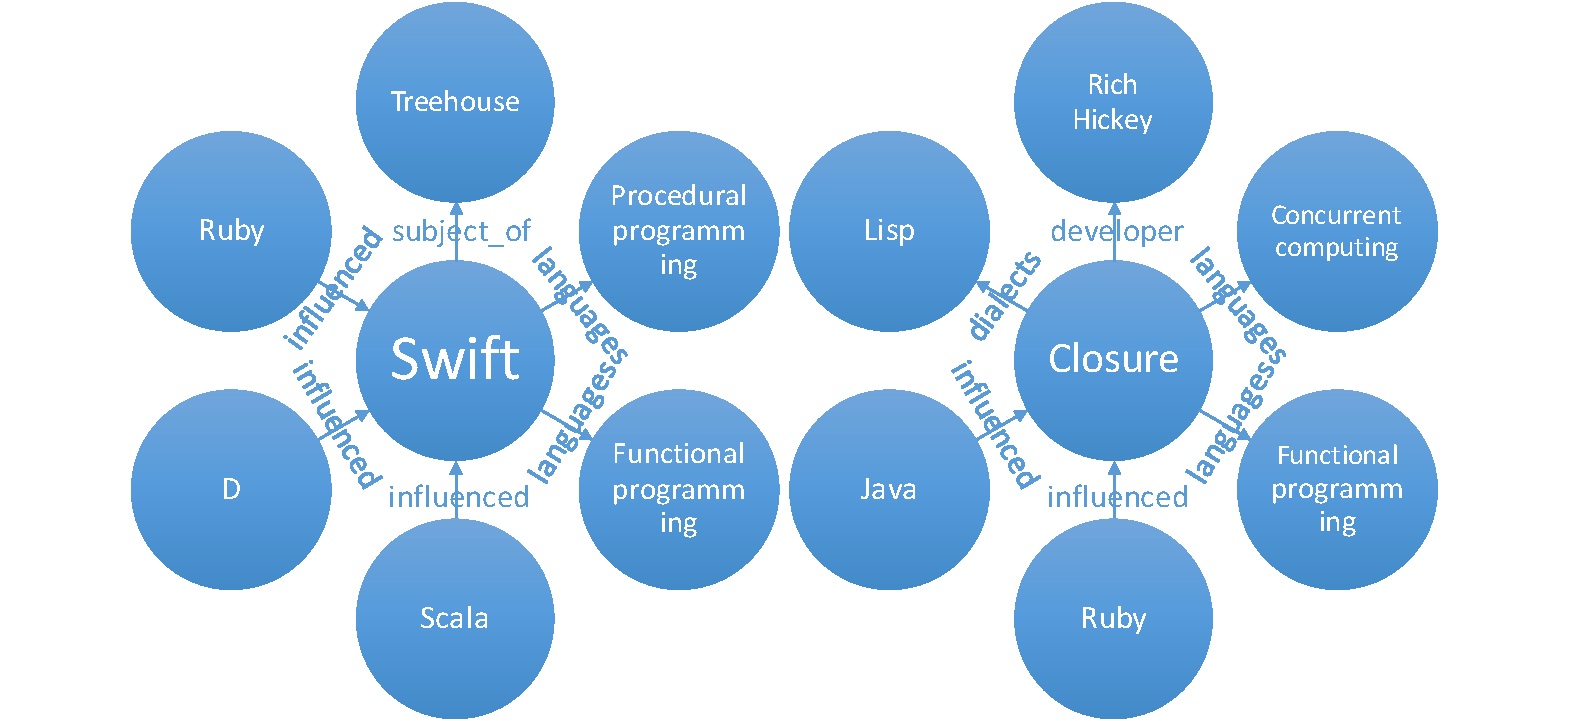
\includegraphics[width=3.5in]{swift.pdf}
\caption{ETEQ and relevant answer}\label{fig:swift-closure}
\end{figure}

\section{Definitions and Problem Statement}
The ``Resource Description Framework'' or RDF\cite{klyne2006resource} is a standard data model for describing Web resources, but it also has become a popular data model for publishing linked data.  RDF encodes Web data as a labeled directed graph using nodes to represent Web resources or entities and edges to represent the links between them.  RDF data can be formally represented as a directed labeled graph. 
\begin{definition}{(RDF Graph)}
An RDF graph $G = \left \langle V, E, L\right\rangle$ is an directed labeled graph, where $V$ denotes a set of nodes, $E \subseteq V^2$ is a set of edges, and $L$ is a labeling function that maps each node in $V$ and each edge in $E$ to a label.
\end{definition}

Unless explicitly stated otherwise, the term graph in this paper refers to a labeled directed graph.

\begin{definition}{(Edge-preserving Isomorphism)}
A graph $G$ is edge-preserving isomorphic to a graph $G'$, denoted as $G\simeq G'$, if there is a bijective function $\mu$ from the nodes of $G$ to the nodes of $G'$ such that for every edge $n_1 \xrightarrow{l} n_{2}$ in $G$, the edge $\mu(n_1) \xrightarrow{l} \mu(n_2)$ in $G'$.
\end{definition}

\begin{definition}{(Edge-preserving Edit Distance)}
The edit distance between two non-isomorphic graphs $G$ and $G'$ is the minimum number of of edit operations that makes $G \simeq G'$. 
\end{definition}

Generally, edit operations include insertion, deletion and substitution of edges or nodes. Our discussions in this paper focus on the substitution of edge labels.  However, our algorithms can easily be extended to support other two edit operations. 

\begin{definition}{(Error-tolerant Exemplar Query)}
An error-tolerant exemplar query is a query that may contain error on the edge labels and may not perfectly match relevant answers. 
\end{definition}

In the rest of paper, we will use the term query for an error-tolerant exemplar query and the relevant answers to denote the query result set. 

\begin{definition}{(Query Cost Model)}
A query cost  model is a parametric equations that estimates the cost of an algorithm or a query plan, in terms of the number of operations (I/O and CPU) that is needed to evaluate the query.
\end{definition}

\noindent {\bf Problem Statement:} We aim to address the following two problems. (1) Given an ETEQ in the form of a query graph $q$ and an edit distance threshold $t$, we aim to efficiently retrieve all relevant answers in a data graph that are edge-preserving isomorphic to $q$ with at most $t$ edit operations. (2) Given two algorithms for the problem in (1), we aim to compare their costs in terms of a cost model and find out the conditions under which one algorithm outperforms the other. 

\section{Exemplar Queries with Edit Distance Constraint}
\subsection{The Basic EXED Algorithm}
Given a data graph $G\,=\,(V,\,E)$, a query $Q$ and the edit distance threshold $t$, the basic exemplar queries with edit distance constraint algorithm (EXED) discovers a set of subgraphs that are within $t$ edit distances of the query $q$. A naive approach is to compare the query with every subgraph in the data graph $G$. Instead of comparing the query with an exponential number of subgraphs in the data graph, EXED randomly chooses one node $n_q$ from the query as a seed. Subsequently, it considers all nodes of the data graph one by one as a possible mappings of the node $n_q$. For each such node $n_g$ in $V$,  it checks if there exists a subgraph that contains $n_g$ and is isomorphic to the query with at most $t$ edit operations. All matching subgraphs are added into the result set. Algorithm 1 describes the above steps in pseudocode.

The algorithm starts from the query subgraph $q$ only containing $n_q$ and a data subgraph $g$ only containing $n_g$, and maps $n_q$ to $n_g$. It iteratively adds edges from $Q$ and $G$ to $q$ and $g$ respectively until $q$ is equal to $Q$ and $g$ is isomorphic to $Q$ with at most $t$ edit operations. 
\begin{algorithm}
\caption{\textproc{EXED}}
\label{EXED}
\begin{algorithmic}[1]
\INPUT Data graph $G=\,\left \langle V,\,E\right\rangle$, query graph $Q$
\INPUT Threshold $t$
\OUTPUT Set of answers $S$
\State $S \leftarrow \emptyset$
\State $n_q \leftarrow chooseARandomNode(Q)$
\For{each node $n_g \in V$}
\State $s\,=\,$ \Call{SearchSimilarSubgraph}{$G$, $Q$, $n_q$, $u$, $t$}
\If{$s\,\not=\emptyset$}
	\State Add $s$ to answer set $S$.
\EndIf
\EndFor \\
\Return $S$
\end{algorithmic}

\end{algorithm} 
\subsection{A Neighbourhood-based Pruning}
In EXED, every node $n_g$ of the data graph is considered a possible match of the query node $n_q$ and as a seed to start the search for relevant answers. However, only a small fraction of data nodes are true candidates, and considering every node of the data graph as a possible match of $n_q$ is highly inefficient.  

To reduce this search space, one has to reduce the number of unnecessary data nodes from which the search for similar subgraphs starts. Inspired by \cite{khan2011neighborhood}, we propose a method called $\textproc{NeighbourhoodPruning}$ to prune the search space.

\begin{definition}{($d$-neighbour)}
\label{d-neighbor}
Let $n \in V$ be a node of the
data graph $G = \left \langle V, E\right\rangle$. The node $n_i \in V$ is a $d$-neighbour
of n if there exists a path from $n$ to $n_i$ of length at
most $d$. The $d$-neighbourhood nodes of n, denoted as $N_d(n)$, is the
set of all $d$-neighbours of $n$, and the $d$-neighbourhood labels of n, denoted as $L_d(n)$, is the
set of edge labels on paths of length at most $d$ from n to its d-neighbour nodes.
\end{definition}

$\textproc{NeighbourhoodPruning}$ compares data nodes with query nodes using their neighbourhood information, and filters out those data nodes that requires more than $t$ edit operations to match the query node's neighbourhood. Let $T_{n, k, l}$ denotes those neighbour nodes of n which are reachable from n in a path of length k and l is the last label in the path, i.e. 
\begin{equation*}
T_{n, k, l} = \left\{n_1 | n_1 \xrightarrow{l} n_2\cup n_2 \xleftarrow{l} n_1, n_2 \in N_{k-1}(n)\right\}.
\end{equation*}

Since keeping the table of neighbour nodes for every data nodes is expensive in term of space, we only keep the cardinality of $T_{n,k,l}$. Also, in order to efficiently retrieve data node candidates for a query node, we implement an inverted index which stores a list of nodes for every label, every cardinality and every distance. In other words, the index allows us to efficiently find data nodes that have a label $l$ at their $k$-neighbourhood with a certain cardinality. 

Once the neighbourhood tables $T_{n, k, l}$ of both data and query nodes are computed for each label $l$ and path length $k \leq d$, then we can compare the neighbourhood of a query node to that of a data node and filter out unqualified data nodes. The edit distance between data node $n_g$ and query node $n_q$ for label $l$ at $k$-neighbourhood can be written as
\[
dist_{k,l}(n_q, n_q)=
\begin{cases}
0 & \text{if } |T_{n_g,k,l}| \geq |T_{n_q,k,l}|\\
|T_{n_q,k,l}| - |T_{n_q,k,l}| &\text{otherwise}.
\end{cases}
\]
Given an edit distance threshold $t$, $n_g$ is considered a candidate for the query node $n_q$ when the distance between the $d$-neighbourhoods of the two nodes does not exceed $t$, i.e.
\[
\sum_{i=1}^d\sum_{l \in L_i(n_q)} dis_{i,l} \leq t.
\]

Note that this filtering may introduce false positives, because neighbourhood-based pruning cannot identify if  the labels are in the same path. For example, this neighbourhood-based distance between query nodes $q_1$ and $g_1$ in Figure~\ref{fig:falsep} is $0$ whereas the actual edit distance is $6$. It may be noted that the more correlated the edge labels in a query's path are, the less false positives the neighbourhood-based pruning can produce. This summarized representation of a neighbourhood is highly effective at pruning nodes without actually visiting their neighbourhood and the false positives can be removed at the verification stage.  

\begin{figure}[H]
\setlength{\belowcaptionskip}{-0.5\baselineskip}
\centering
\begin{forest}
for tree={circle,draw, l sep=10pt}
[$q_1$, 
    [$q_2$, edge label={node[midway,left] {$l_1$}}
      [$q_3$,edge label={node[midway,left] {$l_2$}} ] 
      [$q_4$, edge label={node[midway,left] {$l_3$}}] 
      [$q_5$, edge label={node[midway,right] {$l_4$}}]
    ]
    [$q_3$, edge label={node[midway,right] {$l_5$}}] 
]
\end{forest}
\begin{forest}
for tree={circle,draw, l sep=10pt}
[$g_1$, 
    [$g_2$, edge label={node[midway,left] {$l_1$}}]
    [$g_3$, edge label={node[midway,right] {$l_5$}}      
    [$g_4$,edge label={node[midway,left] {$l_2$}} ] 
      [$g_5$, edge label={node[midway,left] {$l_3$}}] 
      [$g_6$, edge label={node[midway,right] {$l_4$}}]] 
]
\end{forest}
\caption{Query graph and data graph}
\label{fig:falsep}
\end{figure}

At the verification stage, instead of comparing query nodes with data nodes independently and combining the match results, a more efficient approach is to take the previous comparisons of the nodes into the consideration. \begin{definition}{(Simulation)}
Let  $G_1 = \left \langle V_1, E_1\right\rangle$ and $G_2 = \left \langle V_2, E_2\right\rangle$ be two graphs. $G_2$ simulates $G_1$ if there exists  a relation $R$ such that, for every node $n_1 \in N_1$ and $n_2 \in N_2$ for which $(n_1,n_2) \in R$ and $n_1 \xrightarrow{l} n_1'$, there exists a $n_2'$ such that $n_2 \xrightarrow{l} n_2'$ and $(n_1,n_2) \in R$.
\end{definition}

Verifying a simulation can be done more efficiently since $n_{2}^\prime \in V_g$ is a possible match of a query node $n_{1}'$ only if in a previous comparison of nodes $n_{2}$ and  $n_{1}$, $n_{2}$ is identified as a possible match of $n_{1}$ and there is an edge between $n_{2}$ and $n_{2}'$ with label $l$ and a corresponding edge with label $l$ between $n_{1}$ and $n_{1}'$. With this observation, we only need to examine adjacent nodes of previously matched data nodes rather than all data nodes to find possible matches of a query node.  

The EXED algorithm randomly chooses a query node $n_q$ as a seed (starting node) and starts the search from the seed node. However, when we take the previous comparisons of the nodes into consideration, the choice of the starting node can affect the performance of the algorithm. The fewer previously matched data nodes are, the less comparisons we need do in the following steps of the simulation. We implement this by introducing the concept of selectivity into our algorithm. 

\begin{definition}{(Selectivity)}
The selectivity of a query node $n$ is the ratio of $n$'s matches to the number of vertexes in $G$. The selectivity of label $l$ is the ratio of frequency of label $l$ to the number of edges in $G$.
\end{definition}

As the actual selectivity of a query node may be known only after finding its matches, we devise a method to estimate the selectivity in advance. In this section, we assume the selectivities of nodes are known. The selectivity estimation is studied in detail in Section ~\ref{sec:sel}.   

\begin{algorithm}
\caption{\textproc{NeighbourhoodPruning}}
\label{alg:NeighbourhoodPruning}
\begin{algorithmic}[1]
\setcounter{ALG@line}{0}
\INPUT Data graph $G=\,\left \langle V_g,\,E_g\right\rangle$, query graph $Q=\,\left \langle V_q,\,E_q\right\rangle$
\INPUT Threshold $t$
\OUTPUT Set of candidate mappings $\mu \subset V_q \times N_g $ 
\State $L_d^s \leftarrow$ $d$-neighbour labels of $Q$
\State $\text{Vis} \leftarrow \emptyset$
\State $n_{min} \leftarrow \argmin\limits_{n \in V_g} Sel(n)$
\State $N_g \leftarrow (V_g, \vec{0})$ 
\State $\mu(n_{min}) \leftarrow N_g$
\State $Q \leftarrow \{n_{min}\}$
\For {each $n_q \in Q$}
	\If{$ \left \langle n_q, n_{q}' \right\rangle_l\in E_q$ and $n_{q}' \not\in \text{Vis}$}
		\State Update edit distance of nodes in $\mu(n_q)$, $\mu(n_q')$.
		\State Remove nodes that exceed threshold. 
	\EndIf
	\State $Q \leftarrow Q \cup \{n_q' | n_q \xleftarrow{l} n_{q}' \vee n_q \xrightarrow{l} n_{q}' \}$
	\State $Q \leftarrow Q \setminus \{n_q\}$
	\State $\text{Vis} \leftarrow \text{Vis} \cup \{n_q\}$
\EndFor
\end{algorithmic}
\end{algorithm}

Let $n_{min}$ be a query node with the minimum selectivity. The algorithm initially takes the set of all data nodes as candidate mappings candidate of $n_{min}$. For each query node $n_q$ that has not been visited yet, the algorithm checks if each data node $n \in V_g$ has the matching edges (i.e. edges with the same label and direction) for each adjacent edges of $n_q$. If it does not match and the edit distance $t$ has already reached the threshold, $(n, t)$ is removed from $\mu(n_q)$. If it does not match and $t$ has not reached the threshold, a node $n'$ adjacent to $n$ is considered  as a candidate for the query node $n_q'$ adjacent to $n_q$ and the entry $(n',t+1)$ is inserted into $\mu(n_q')$. Otherwise,  $n'$ is a the candidate of $n_q'$with no edit penalty and the entry $(n',t)$ is inserted into $\mu(n_q')$. Finally, the query node $n_q$ is marked as visited and is removed. Algorithm 2 describes the pseudocode of above steps. 

\subsection{Speeding up Neighbourhood-based Solution}
The neighbourhood-based filtering may introduce false positives, because two matching labels may not be under the same path or have the same direction. In this section, we introduce a path-based filtering algorithm to prune out some of the false positives.

The path-based filtering algorithm compares data nodes with the query node in terms of their paths and filters out those data nodes that requires more than t edit operations to match the query node. However, keeping every path for every node can be very expensive in term of space. For a graph with average degree $\hat{D}$ and $d$-edge path indexes, the space required for using path indexes is $O(\hat{D}^d)$. Our approach to reduce the space is using the Bloom filter\cite{bloom1970space}.  

A Bloom filter is a space-efficient probabilistic data structure to efficiently test whether an element is a member of a set $N$. An empty Bloom filter is a bit array of $m$ bits, all set to $0$. There are $k$ different hash functions, each mapping an element to one of the $m$ array positions. To query for an element, one needs to find the $k$ array positions the element is mapped to. If any of the bits at these positions is 0, the element is definitely not in the set. If all are 1, then either the element is in the set, or the bits have by chance been set to $1$ during the insertion of other elements, resulting in a false positive. The error rate $p$ depends on $m$, $|N|$ and $k$.We set the false positive rate to  $1\%$. The optimal number of hash functions is approximately $0.7m/|N|$, and the optimal number of bits $m$ is approximately $|N|\ln{p}/\ln^2{2}$. The number of inserted elements can be estimated by $\hat{D}^d$, where $\hat{D}$ is the average degree of the data graph\cite{chazelle2004bloomier}.  The Bloom filter based path filtering allows us to control the false positives at a low rate with a compact storage and an efficient access time. Moreover, it has no false negatives. 

To insert a path into the Bloom filter, we concatenate the labels in the path to form a string that is inserted into the Bloom filter.  To encode the direction of an edge, a sign symbol is added to each label to distinguish between incoming and outgoing edges. In addition, the count of each path is described by preceding the label sequence and separated from the rest of string by ``P''. For example, the string ``2P+1-2'' describes two paths that have one outgoing edge labeled with value $1$ and one incoming edge labeled with value $2$. Since all labels in a path are encoded into one string, an unmatched path can have up to $d$ unmatched labels. To avoid filtering out false negatives, we consider the lower bound of the edit distance for an unmatched path, which is $1$. This also introduces false positives if we only use path filtering. However, these false positives can be removed by considering the neighbourhood filter.  

Our experiments show that the two filtering schemes work nicely, complementing each other. This is because path filtering can identify if multiple labels are in the same path and if the matching edges with the same labels have the same direction which neighbourhood filter cannot do; on the other hand, neighbourhood filtering can identify the level of mismatched labels which cannot be done by a path-based filtering.
\subsection{A Wildcard Solution}
The main problem with EXED is that the number of intermediate results can become huge, especially for large edit distance thresholds and large node degrees of the data graph. Most of those intermediate results need to be kept until a very late stage of the searching.  

To reduce the number of intermediate results, we develop a new algorithm referred to as wildcard queries with edit distance constraint (WCED). The approach taken in this algorithm is to map the subgraph edit distance problem instance into subgraph isomorphism problem instances without missing any relevant answers. This is done by introducing the concept of wildcard labels. 
\begin{definition}{(Wildcard Label)}
A wildcard label is a label that can substitute for any other label in graph matching.
\end{definition}

The main idea is to perform multiple subgraph isomorphism searches based on the original query and merge the retrieved answers to obtain the final results. This approach has two phases: query pre-processing and subgraph search and answer mergence. 

In the query preprocessing phase, we choose $t$ edges from $|E_q|$ query edges, where $t$ is the edit distance threshold and set their labels to the wildcard label. This gives us ${|E_q| \choose t}$ wildcard queries assuming that $t \leq |E_q|$. For example, Figure~\ref{fig:wcq} shows a two-edge query and its wildcard queries with edit distance threshold $1$. 

In the next phase, we run subgraph isomorphism searches on those generated wildcard queries. For this, we directly adopt EXED with edit threshold set to $0$. This returns the subgraphs where the wildcard matches any labels. For example, searching for the first wildcard query in Figure~\ref{fig:wcq} will give us all subgraphs which have an edge labelled $l_1$ and and an edge with any label, both under the same parent node. Finally, duplicates due to possible overlappings between wildcard queries are removed. 

The WCED algorithm reduces the number of intermediate results by converting the subgraph edit distance into subgraph isomorphism. This is for the cost of running EXED ${|E_q| \choose t}$ times with edit distance threshold $0$. 

Another advantage of using WCED is that it can be easily extend to handle other edit operations, such as insertion and deletion (as discussed next). 

{\bf Supporting deletions} This is similar to substitution except that the edges are removed instead of being labeled with a wildcard. With $|E_q|$ query edges and edit distance threshold t, there are ${|E_q| \choose t}$ possible choices for deletion, each leading to a subgraph isomorphism search. 

{\bf Supporting insertions} Since we are searching for subgraphs of the query graph, insertions are already supported at no cost. For example, the data graph can have any number of additional edges, and those edges are ignored in a subgraph search (and there is no need to insert query edges).

\begin{figure}[H]
\setlength{\belowcaptionskip}{-0.5\baselineskip}
\centering
\begin{forest}
for tree={circle,draw, l sep=10pt}
[$q_1$, 
    [$q_2$, edge label={node[midway,left] {$l_1$}}]
    [$q_3$, edge label={node[midway,right] {$l_2$}}] 
]
\end{forest}
\begin{forest}
for tree={circle,draw, l sep=10pt}
[$q_1$, 
    [$q_2$, edge label={node[midway,left] {$l_1$}}]
    [$q_3$, edge label={node[midway,right] {$*$}}] 
]
\end{forest}
\begin{forest}
for tree={circle,draw, l sep=10pt}
[$q_1$, 
    [$q_2$, edge label={node[midway,left] {$*$}}]
    [$q_3$, edge label={node[midway,right] {$l_2$}}] 
]
\end{forest}
\caption{Query graph and its wildcard queries}
\label{fig:wcq}
\end{figure}

%\begin{figure}[H]
%\centering
%\tikzset{
%% Two node styles for game trees: solid and hollow
%solid node/.style={circle,draw,inner sep=1.5,fill=black},
%hollow node/.style={circle,draw,inner sep=1.5}
%}
%\begin{tikzpicture}[scale=1.5,font=\footnotesize]
%% Specify spacing for each level of the tree
%\tikzstyle{level 1}=[level distance=8mm,sibling distance=8mm]
%% The Tree
%\node(0)[hollow node, label=above:{$1$}]{}
%child{node[hollow node,label=below:{$2$}]{} edge from parent[->] node[left]{$a$}}
%child{node[hollow node,label=below:{$3$}]{} edge from parent[->]  node[right]{$b$}}
%;
%\end{tikzpicture}
%  % Node styles
%\tikzset{
%% Two node styles for game trees: solid and hollow
%solid node/.style={circle,draw,inner sep=1.5,fill=black},
%hollow node/.style={circle,draw,inner sep=1.5}
%}
%\begin{tikzpicture}[scale=1.5,font=\footnotesize]
%% Specify spacing for each level of the tree
%\tikzstyle{level 1}=[level distance=8mm,sibling distance=8mm]
%% The Tree
%\node(0)[hollow node, label=above:{$1$}]{}
%child{node[hollow node,label=below:{$2$}]{} edge from parent[->] node[left]{$a$}}
%child{node[hollow node,label=below:{$3$}]{} edge from parent[->]  node[right]{$*$}}
%;
%\end{tikzpicture}
%\tikzset{
%% Two node styles for game trees: solid and hollow
%solid node/.style={circle,draw,inner sep=1.5,fill=black},
%hollow node/.style={circle,draw,inner sep=1.5}
%}
%\begin{tikzpicture}[scale=1.5,font=\footnotesize]
%% Specify spacing for each level of the tree
%\tikzstyle{level 1}=[level distance=8mm,sibling distance=8mm]
%% The Tree
%\node(0)[hollow node, label=above:{$1$}]{}
%child{node[hollow node,label=below:{$2$}]{} edge from parent[->] node[left]{$*$}}
%child{node[hollow node,label=below:{$3$}]{} edge from parent[->]  node[right]{$b$}}
%;
%\end{tikzpicture}
%\caption{Original query and its wildcard queries}
%\end{figure}

\section{Algorithm Cost Analysis}
In the previous sections, we presented two algorithms for exemplar queries with edit distance constraints, each with some advantages over the other. WCED has much less number of intermediate results (meaning less space usage), while EXED only needs to be run once and has no duplicate answers. To determine which algorithm has the least cost for a given query and data graph (without actually running the algorithms), one needs an accurate cost estimation. This is the problem addressed in this section. 

EXED consists of three parts: starting node selection, neighbourhood-based pruning and subgraph verification.  The time cost of starting node selection and  neighbourhood-based pruning are linear in the number of query nodes and number of data graph nodes respectively, while the time cost of subgraph verification grows exponentially with the edit distance threshold and the number of query edges. WCED consists of three phases: query pre-processing, subgraph isomorphism search and answer mergence. Subgraph isomorphism search uses EXED  with the edit distance threshold $0$, the cost of which also grows exponentially with the number of query edges. The time cost of query pre-processing depends on the number of query edges and the edit distance threshold. The time cost of  answer mergence is linear in the number of answers. Both of them are relatively low and negligible compared to the cost of subgraph isomorphism search. Therefore, we focus on the cost of  verification of two algorithms. The cost depends on the number of data nodes (candidates) matching the query starting node and the cost of verifying each candidate. 

In this section, we first present an estimation for the selectivities of edge labels. We then present an exact cost model and an upper-bound cost model. 

\subsection{Selectivity Estimation}
\label{sec:sel}
The probability that an arbitrary edge in the data graph has label $l$, referred to as the selectivity of label $l$, can be written as
\begin{align*}
Sel(l)  = \frac{freq(l)}{|E_g|}
\end{align*}
where $freq(l)$ is the frequency of label $l$ in the data graph $G$, and $|E_g|$ is the number of edges in $G$.
\subsection{An Exact Cost Model} 
Both algorithms EXED and WCED start with a set of candidate nodes in data graph $G$ that are likely to match a query node $n_s$; those candidates may be selected based on a filtering scheme such as the neighbourhood or the path filtering. 
Given a candidate node in $G$, we must check if there is a subgraph in $G$ that simulates the query graph in which the candidate node matches $n_s$. 
The cost of this process depends on two factors: the number of candidates matching the query node and the cost of verifying each candidate. 
\subsubsection{A cost model for WCED}
Given a query and an edit distance threshold that is larger than zero,
the WCED algorithm generates a set of wildcard queries based on the edit distance threshold, hence it has to perform multiple subgraph isomorphism searches on those wildcard queries.
To estimate the cost, we need to estimate the cost of each search and sum up the costs. It should be noted that a wildcard query is like any query except that some edges are labeled with wildcards and those wildcards can match any label.

\noindent {\bf Estimating the number of candidates:}
Given a seed $n_s$, we want to estimate the probability that a data node is a candidate for $n_s$. 

%\begin {lemma}
%\label{lemma:pl1-k}
%Given a query node with edges in its 1-neighbourhood labeled $l_1, l_2, \ldots, l_k$, the probability that a data node of degree $D$ has all those edge labels is
%\begin{align}
%\label{eq:pl1-k}
%P(l_1, l_2, ..., l_k) &= P(l_2, l_3, ...,l_k) + \sum_{i=2}^k (-1)^{i-1} * P (K_i) \\ \nonumber
%&+ (-1)^k P(\neg l_1, \neg l_2, ..., \neg l_k)
%\end{align}
%where
%\[
%P(K_i) = P(\neg l_1,  ..., \neg l_{i-1}, l_{i+1}, ..., l_k)\ \  for\ \ 1\leq i \leq k.
%\]
%\end{lemma}
\begin {lemma}
\label{lemma:pl1-k}
Given a query node and its adjacent edge labels $l_1, \ldots, l_k$, and assuming independence between the labels, the probability that a data node with $D$ adjacent labels has all query labels is
\begin{align}
\label{eq:pl1-k}
&P_D(l_1, l_2, ..., l_k) =  \\ \nonumber
&\sum_{j=1}^{k-1} \sum_{i=j+1}^k (-1)^{i-1}P_D(\neg l_j,\ldots,\neg l_{i-1}, l_{i+1}, \ldots, l_k) +\\ \nonumber
&\sum_{j=1}^{k-1} (-1)^{k-j+1}(1-\sum_{i=j}^k Sel(l_i))^D + (1-(1-Sel(l_k))^D.
\end{align}
\end{lemma}

See the extended version of this paper \cite{eteq2016} for a detailed proof. 
Lemma~\ref{lemma:pl1-k} directly gives the selectivity of a query node based on its 1-neighbourhood.
Let $L_i(n_q)$ denote the set of labels at the $i^{th}$ neighbourhood of a query node $n_q$.
%Let $L_{nq}^d$ denote the set of labels of a query node $nq$ at levels $1$ to $d$.
The probability that the neighbourhood of a data node matches that of a query node at levels $1, \ldots, d$
can be written as 
\begin{equation}
\label{eq:plm1-d}
P(n_q) =\prod_{m = 1}^dP_{D_m}(L_m(n_q)). 
\end{equation}
where $P_{D_m}(L_m(n_q))$ is as defined in Lemma~\ref{lemma:pl1-k} and $D_m$ is the number of edges at the $m^{th}$ neighbourhood of a data node.
We generally don't know $D_m$ when estimating our probabilities in Equations~\ref{eq:pl1-k}.
Assuming that each data node has the same degree $\hat{D}$, then $D_m=\hat{D}^m$. 
%Let $D_{avg}$ and $D_{avg}^m$ denotes the number of distinct labels at levels $1$ and $m$ respectively.
Then, we can have the number of candidates matching query node $n_q$ as 
\begin{align*}
|C(n_q)| = |V_g| * P(n_q).
\end{align*}

\noindent {\bf Estimating the cost of verifying each candidate:}
For each candidate of the starting node, the algorithm starts from a graph $g$ with only one node (i.e. the candidate node) and iteratively adds new edges to $g$ until either $g$ simulates the query, or no such simulation is found.
%% we need the algorithm to refer to in our cost estimation
%This is done by iterating over the query edges, retrieving the matching edges and their adjacent nodes from the data graph, and joining the results. 
The cost of adding each new edge depends on the expected number of matching edges of a query edge and the number of subgraphs to which the edges are added.
Let $\hat{D}$ denote the expected degree of a data node.
For a query label $l_i$, we expect $\hat{D}*Sel(l_i)$ edges of a node in the data graph to match $l_i$. 
For a fixed candidate node in the data graph, the expected number of subgraphs (partial matchings) that can be constructed starting from the candidate and simulating the query subgraph rooted at the seed with labels $l_1, \ldots, l_k$ is 
\[
\prod_{i=1}^{k}\hat{D}*Sel(l_i). \nonumber
\]
and the total expected cost of verifying a candidate $n$ is
\begin{equation}
\label{eq:cost-verifying-n}
\sum_{i=1}^{|E_q|}\prod_{j = 1}^i\hat{D}*Sel(l_j).
\end{equation}
%
Note that this is based on the assumption that a search starting from a candidate node will not stop early if the simulation exceeds the edit distance threshold. 

The total cost of verifying $|C(n_q)|$ candidates for possible matches to query $q$ is
\begin{equation}
\label{eq:cost-verifying-q}
Cost(q) = |C(n_q)| * \sum_{i=1}^{|E_q|}\prod_{j = 1}^i\hat{D}*Sel(l_j).
\end{equation}
  
Since we have replaced a query graph with ${|E_q| \choose t}$ graphs each with $t$ wildcards, the total cost is the sum of the costs of verifying those wildcard queries.

%\begin{align*}
%Cost_{wc} = \sum_{i=1}^{{|E_q| \choose t}}Cost(wcq_i)
%\end{align*}

\subsubsection{EXED Cost Model}
To estimate the cost for  EXED, we also need to estimate  the number of candidates in the data graph matching a query seed node and the cost of verifying each candidate. 

\noindent {\bf Estimating the number of candidates:} 
Since a data node is allowed to have up to $t$ edit operations in its neighbourhood, directly estimating the probability that a data node is a qualified candidate is difficult. Therefore, we estimate the number of candidates for a set of wildcard queries where the labels are all fixed. 
By summing up the number of candidates for these wildcard queries and removing the repetitive candidates due to overlaps between queries,  the number of candidates for $n_q$ in EXED can be written as
\begin{align}
\label{eq:Cnq}
|C(n_q)| &= \sum_{i=1}^{|E_q| \choose t}|V_g| * P(n_{w_i(q,t)}) \nonumber\\
&- ({|E_q| \choose t} - 1) * |V_g| * P(n_q).
\end{align}
where $w_i(q,t)$ is a wildcard query constructed from $q$ by replacing $t$ edge labels with wildcards
and $P(n_q)$ is as in Equation~\ref{eq:plm1-d}. With $t$ edit operations, the number of wildcard queries is ${|E_q| \choose t}$ and the last term gives the number of double-counts.

\noindent {\bf Estimating the cost of verifying each candidate:}
To estimate the cost of verifying each candidate, we need to estimate the number of partial matchings.
There are two kinds of partial matchings in EXED: (1) those matchings that have reached the edit distance threshold; (2) those matchings that have not reached the threshold. For those partial matchings that have not reached the threshold, edges with any label can be added to the matching in the next step of the simulation, whereas for those matching that have reached the threshold, only edges with matching labels can be added. Let $m$ be the number of edges in a partial matching, and $k$ be the number edges in the matching where the matching edges have different labels. If $l_1, \ldots, l_k$ denote the query labels in the matching where the labels don't match, and $l_{k+1}, \ldots, l_m$ be the
labels where both data and query edges in the matching have the same labels,
then the number of partial matchings can be written as
\[
\hat{D}^m \prod\limits_{i=1}^{m-k}Sel(l_i)\prod\limits_{j=1}^{k}(1-Sel(l_j)).
\]
Given query labels $l_1, \ldots, l_m$, we generally don't know in advance which labels will mismatch and need to check all choices of ${m \choose t}$ sets of labels. The number of partial matchings that needs to be verified is 
\begin{equation}
\label{eq:st-cases}
    S_t(q,m)= 
\begin{cases}
    0         			  & \text{if } t > m\\
    \hat{D}^m\prod\limits_{i=1}^{m}Sel(l_i) & \text{if }t=0\\
    \sum\limits_{k=1}^{m \choose t}\hat{D}^m \prod\limits_{i=1}^{m-t}Sel(l_{k,i})\prod\limits_{j=1}^t(1-Sel(l_{k,j}))& \text{if } t < m.
\end{cases}
\end{equation}

For those partial matchings that have not reached the threshold $t$, any edge can be added into those partial matchings in the next step of the simulation. In this case, the next step of simulation costs
\[
\sum\limits_{j=0}^{t-1}S_j(q,m) * \hat{D}.
\]

For those partial matchings that have reached the threshold, only edges with a matching label can be added into those partial matchings. In this case, the next step of simulation costs
\[
S_t(q,m) * \hat{D} * Sel(l_{m+1}).
\]

The cost of verifying each candidate in  EXED can be written as
\begin{align}
\label{eq:ed-verify}
Cost(q) = \sum\limits_{i=0}^{|E_q|-1}(S_t(q,i) * \hat{D} *  Sel(l_{i+1}) + \sum\limits_{j=0}^{t-1}S_j(q,i) * \hat{D}).
\end{align}

The total cost of  EXED is the product of the number of candidates (as given in Equation~\ref{eq:Cnq}) and and the cost of verifying a candidate (as given above). 
\begin{align*}
Cost_{ex} = |C(n_q)|Cost(q).
\end{align*}

\subsubsection{Cost Model Comparison}
%From the cost models above, we know that $\textproc{EXED}$ and $\textproc{WCED}$ have the same cost  when edit distance threshold $t$ is not less than the number of query edges $|E_q|$. This is because each step of the simulation costs $\hat{D}$ for both $\textproc{EXED}$ and $\textproc{WCED}$ when there are more than $|E_q|$ edit operations allowed. Therefore, we only compare the costs of two algorithms when $t < |E_q|$. In this section, we compare the costs between $\textproc{EXED}$ and $\textproc{WCED}$ using cost models given in previous sections and show that $\textproc{EXED}$  costs less $\textproc{WCED}$ under certain conditions.
%\begin {lemma}
%\label{lemma:comp}
%Given a data graph with large average node degree $\hat{D}$, a query graph $q$ with at least 2 edges and edit distance threshold 1, $\textproc{EXED}$ costs less than $\textproc{WCED}$ when
%\begin{align}
%\label{ineq:constraint}
%Sel(l_1) > \frac{1}{\sqrt[|E_q|]{\hat{D}}}.
%\end{align}
%where $l_1$ is the label that has the highest selectivities in query labels.
%\end{lemma}
%\begin{proof}
%In a data graph $G$ with large $\hat{D}$, every data node has a large number of edge labels and thus is qualified to be candidates of any query seed node. The number of candidates for query seed node in $\textproc{EXED}$ and $\textproc{WCED}$ are both approximately equal to $|V_g|$. In this case, to compare the costs of $\textproc{EXED}$ and $\textproc{WCED}$, we only have to look at the cost of verifying each candidate. 
Our cost comparison assumes that the edit threshold $t$ is less than the number of query edged; otherwise, the problem is subgraph isomorphism with no label constraints, which is not addressed in this paper. 
With that assumption, we want to compare the costs of verifying the candidates for EXED and WCED and find out the conditions under which one outperforms the other.

When the edit distance threshold is larger than zero, the cost of verifying a candidate in EXED is higher than that in WCED, because edit operations can happen on any label in EXED while they are fixed in WCED. In this case, when the number of candidates for WCED and EXED are roughly the same, WCED will outperform EXED. In other words, WCED outperforms EXED if the number of candidates for the original query is small (See Equation~\ref{eq:Cnq}). With few candidates we expect to have fewer isomorphic matches, and this a scenario studied in this paper where matches with edit distance larger than zero are relevant. The next lemma shows what happens when this condition does not hold.
%An interesting question is how the two algorithms perform when this condition does not hold. The following lemma tells us when EXED can outperform WCED with certain constraints.

\begin {lemma}
\label{lemma:comp}
Given a data graph with expected node degree $\hat{D}$, a query graph $q$ with at least $2$ edges and the edit distance threshold set to $1$, 
the cost of verifying a candidate in EXED is less than the sum of the cost of verifying a candidate for every wildcard queries in WCED when
\begin{align}
\label{ineq:constraint}
Sel(l_1) > \frac{1}{\sqrt[|E_q|]{\hat{D}}}.
\end{align}
where $l_1$ is a query label that has the highest selectivity (i.e. the smallest value of $Sel(l_i)$).
\end{lemma}

See the extended version of this paper \cite{eteq2016} for a detailed proof. 
When the number of candidates for the original query is very large and is approximately equal to the number of candidates for each wildcard query, the cost of EXED and WCED can both be approximated by  the number of candidates for the original query and the cost of verifying each candidate. In this case, EXED can outperform WCED given the condition of the lemma.
%If the numbers of candidates for WCED and EXED are equal or approximately equal, using this lemma can give us the condition when one algorithm outperforms the other. There are two cases when the two algorithms have approximately the same number of candidates: (1) the degree $\hat{D}$ is larger than the number of labels in the data graph, in which case, every label will appear in a node's neighbourhood and every node will be a candidate for the query starting node; (2) every pair of labels in the query is highly correlated, in which case, replacing any label of the query does not change the selectivity of the query node; thus the number of candidates is the same for both algorithms.

%
%An interesting question is how the two algorithms perform when the condition of the lemma does not hold. We know that WCED is expected to perform better for queries with low selectivities. In particular, our empirical results show that for queries with two edges, WCED either outperforms or is comparable to EXED when the condition does not hold. Proving this or similar results when the condition of the lemma does not hold is an interesting open problem.

\subsection{An Upper Bound Cost Model}
\label{sec:ub}
The exact cost model is based on two assumptions: (1) labels are evenly distributed, and (2) labels are pairwise independent. These assumptions may not stand in real-world data graphs. The error due to these two assumptions will accumulate and become significant as the number of query edges increases. In this case, we need another cost estimation to deal with larger queries.

In this section, we present a cost model that gives an upper bound of the actual cost but is more accurate for larger query graphs. 
%upper-bound cost models using the data graph's statistical information. Similarly,  we need to estimate the upper bound for the number of candidates and the cost of verifying each candidate.  

\noindent {\bf Estimating the number of candidates:} 
To estimate the upper bound for the number of candidates, two weaker assumptions of label independence are considered: (1) the labels of the adjacent edges of a data node are independent whereas labels, which are in a path starting from a node, are correlated; (2) the labels of the adjacent edges of a data node are correlated whereas labels, which are in a path starting from the node, are independent. For two or more correlated labels, the selectivity of the label with the least selectivity provides an upper bound of the selectivity of the set. 
%This is because using the selectivities of one label instead of every label in a path or adjacent edge labels reduce the selectivity of the path. 

Under the first assumption, the selectivity of the label with the minimum selectivity in each path is used  to estimate the selectivity upper bound of the path. This reduces each path in the query to an edge (with the minimum selectivity), and as a result the query becomes a node with a set of adjacent edges (i.e. a tree with only one level). Assuming independence between the labels of these edges, Lemma~\ref{lemma:pl1-k} will give an upper bound of  the probability that a data node is a candidate for a query node. Note that $D$ in the Lemma is set to the number of paths in the $d$-neighbourhood. 


Under the second assumption, all edges under a node are collapsed into a single edge, which is labeled with a label from the set that has the least selectivity. Since the edge labels of the resulting query are all independent, Equation~\ref{eq:plm1-d} can be used to estimate the upper bound. 

%To compute the upper bound of the candidates number, we simply multiply the probability upper bound by the number of data nodes.

\noindent {\bf Estimating the cost of verifying each candidate: }
To estimate the upper bound for the cost of verifying each candidate, the maximum frequency of each label under a node is used to upper bound the number of matching label in each step of the simulation. 
Let $N(l_i)$ denote the maximum frequency of label $l_i$ in the adjacent edges of a node. 

In our exact cost model, the number of matching labels for a  label $l_i$ is $\hat{D}*Sel(l_i)$ assuming that every label is uniformly distributed on the adjacent edges of a node. Replacing $\hat{D}*Sel(l_i)$ in Equations~\ref{eq:cost-verifying-q} and~\ref{eq:ed-verify} by $N(l_i)$ will give us an upper bound of the cost of verifying each candidate in WCED and EXED respectively. 

\begin{comment}
\begin{figure*}
\centering
\subfigure[the first subfigure]{
\begin{minipage}[b]{2in}
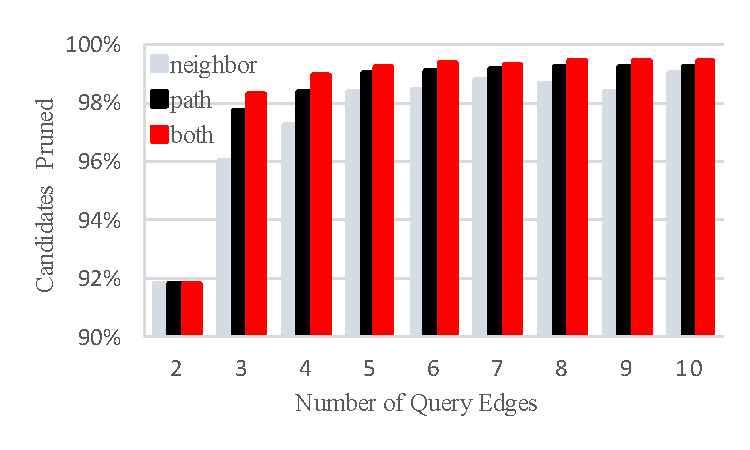
\includegraphics[width=2in]{wcprune.pdf}
\end{minipage}
}
\subfigure[the second subfigure]{
\begin{minipage}[b]{2in}
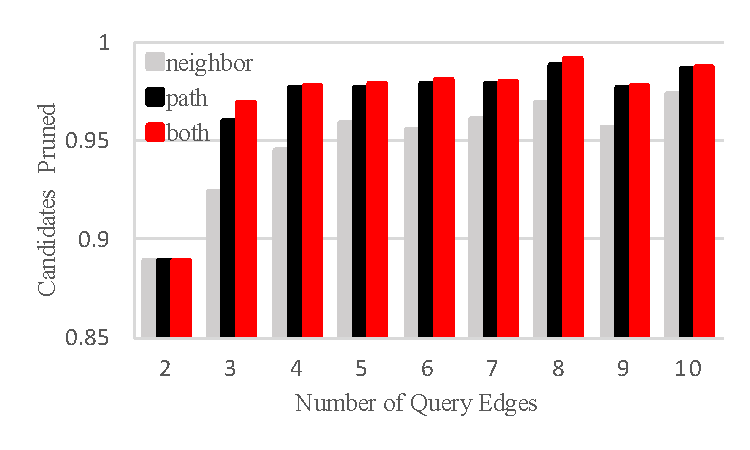
\includegraphics[width=2in]{edprune.pdf}
\end{minipage}
}
\end{figure*}
\end{comment}

\section{Experimental Evaluation}
This section presents an experimental evaluation of our algorithms and cost models. All experiments were performed on a 2.4 GHz 4 Core CPU with 60G memory running Linux. The algorithms are implemented in Java 1.8. In our experiments, unless explicitly stated otherwise, the path length $d$ in our filtering scheme is set to $3$.

\noindent {\bf Dataset:} 
We downloaded a full dump of Freebase\footnote{https://developers.google.com/freebase/} in May 2015. We removed the triples that were used as internal specification for the community (e.g. user and group data and discussion topics) obtaining a fully connected graph of $84$ million nodes and $335$ million edges . Since the entire Freebase is too large for our machine (occupies approximately $90$G of memory when fully loaded), we extract subgraphs from Freebase with different parameters. The subgraphs are extracted using a breadth first traversal of the graph from a randomly selected starting node and randomly choosing new edges to be included in the data graph.  Unless explicitly stated otherwise, the data graphs are randomly generated from Freebase with the number of nodes set to $10$K and average node degree set to $15$.
\begin{comment}
To evaluate the effectiveness of our pruning scheme, we generate synthetic datasets with $50$K nodes having various average degrees. To test the scalability with respect to the graph size, we generate synthetic datasets with are generated $1$K, $10$K, $50$K, $100$K, $500$K nodes having up to $10$M edges.  
\end{comment}

\noindent {\bf Queries:} 
Two types of queries are used in our experiments: (1) A set of real queries from the AOL query log, manually mapped to the data graph, and (2) randomly selected subgraphs of the data graph. These queries vary in the numbers of edges and the selectivities of their labels. Unless explicitly stated otherwise, our experiments use $100$ randomly selected queries, each a subgraph of the data graph. 

\noindent {\bf Summary of our experiments:} 
Section~\ref{sec:filtering} evaluates the effectiveness of our filtering schemes under different parameter settings. The impact of our filtering schemes on the performance of our algorithms and improvements over existing algorithms are evaluated in Sec~\ref{sec:comp}. In Section~\ref{sec:cost}, we evaluate our cost models by studying the correlation between our estimated costs and the real costs.   

\subsection{Effectiveness of Our Cost Models}
\label{sec:cost}
In this section, we evaluate our cost models in terms of the correlation between our estimates and the actual costs. Our results show that: (1) the selectivity estimation is reliable when the number of query edges $|E_q| \leq 10$; (2) there is a linear relationship between our exact cost model and the real cost for $|E_q| \leq 3$ , which allows us to estimate the running time of our algorithms; (3) the exact cost is reliable for the comparison of our algorithms when $|E_q| \leq 6$; (4) the exact cost is reliable for the comparison of query costs when $|E_q| \leq 8$. 

\subsubsection{Effectiveness of the selectivity estimation}
Since selectivity estimation is a core component of our cost model, we first assess the quality of our selectivity estimation. To do so, we measure the correlation between the actual number of candidates and the estimated number of candidates using the selectivity. In our case, the selectivity is  used in choosing a query starting node and for cost comparisons, hence, a relative ordering of the selectivity values is sufficient in theses cases. Therefore, we chose Spearman's rank correlation between estimate and actual selectivities, which shows the monotonic relationship of the two variables. The experiments are in the context of  WCED and EXED algorithms. Let ``exact'' denote the exact selectivity estimation, ``ub-path'' and ``ub-adj'' denote the upper bound of the selectivity estimations respectively assuming that path labels and adjacent labels are independent. Figure \ref{fig:sels} shows that although ``exact'' has the better correlation ($0.96$) than ``ub-adj'' and ``ub-path'' for queries with $2$ edges, the correlation decreases rapidly for queries with a large number of edges, with about 0.55 correlation for queries with $10$ edges. In contrast, the upper-bound selectivity estimations remain stable with different numbers of query edges in both WCED and EXED (with correlation between $0.7$ and $0.96$ and significance level between $3.08E-64$ and $5.38E-16$).  We conclude that there is strong positive correlation between the selectivity estimation and the actual selectivity and that we can safely use this selectivity estimation for the choice of a query starting node and cost comparisons.
\begin{figure}[htb]
\setlength{\belowcaptionskip}{-1\baselineskip}
\centering
\subfigure{
\centering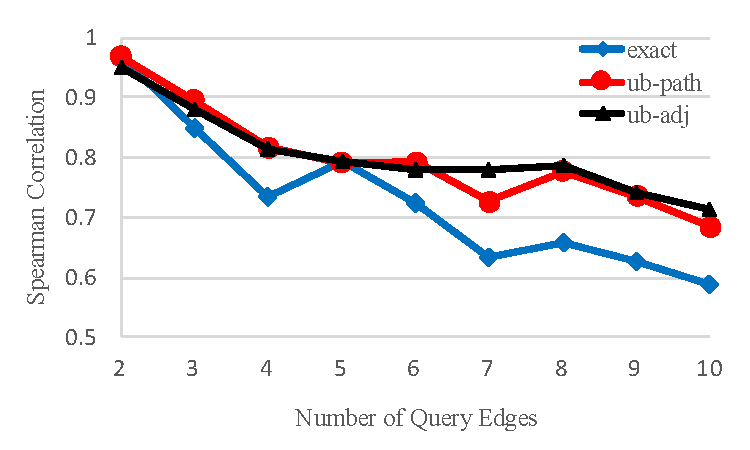
\includegraphics[width=3in]{wc_sels.pdf}
}
\vspace{-2\baselineskip}

\subfigure{
\centering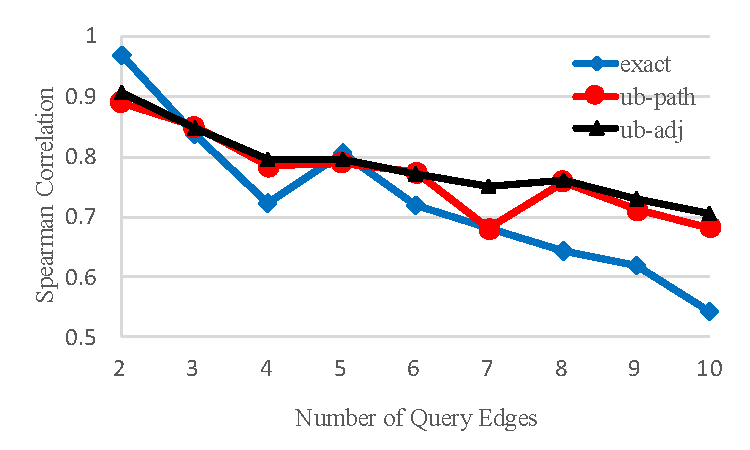
\includegraphics[width=3in]{ed_sels.pdf}
}
\vspace{-2\baselineskip}
\caption{Correlation between estimated and actual selectivities for WCED (top) and EXED (bottom)}
\label{fig:sels}
\end{figure}

\subsubsection{Exact cost model evaluation}
In this set of experiments, we examine the linear relationship between our estimated cost  and the actual number of operations using Pearson correlation. The larger absolute value of the coefficient, the stronger the relationship between the actual cost and the estimated cost. If the absolute value of coefficient  is large, with  simple linear regression, we can predict the actual cost from our estimated cost. Figure ~\ref{fig:exact-cost} shows that for small queries (with up to $3$ edges), the correlation coefficient is over $0.7$ and $0.6$ for WCED and EXED respectively. However, the correlation coefficient drop sharply as the number of edges increases. These results are expected because the exact cost model is based on the assumption that the labels are evenly distributed and that they are independent.
\begin{figure}[htb] 
\setlength{\abovecaptionskip}{-0.5\baselineskip}
\setlength{\belowcaptionskip}{-0.5\baselineskip}
\centering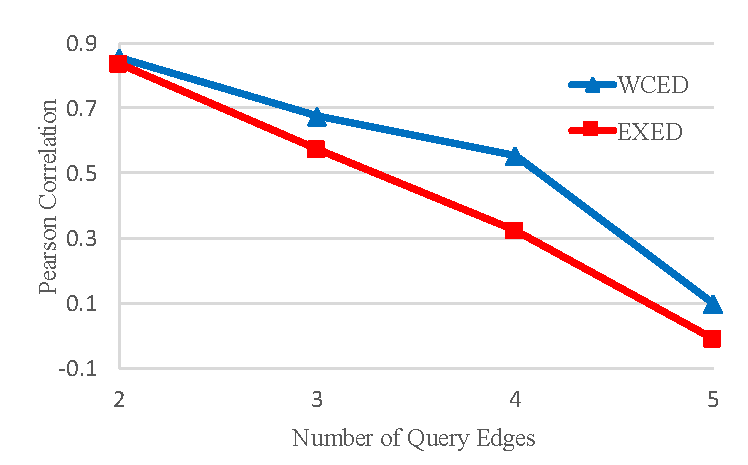
\includegraphics[width=2.5in]{exact_cost.pdf} 
\caption{Correlation between estimated and actual costs varying the number of query edges}
\label{fig:exact-cost}
\end{figure}

\begin{figure}[htb] 
\setlength{\abovecaptionskip}{-0.5\baselineskip}
\setlength{\belowcaptionskip}{-1.5\baselineskip}
\centering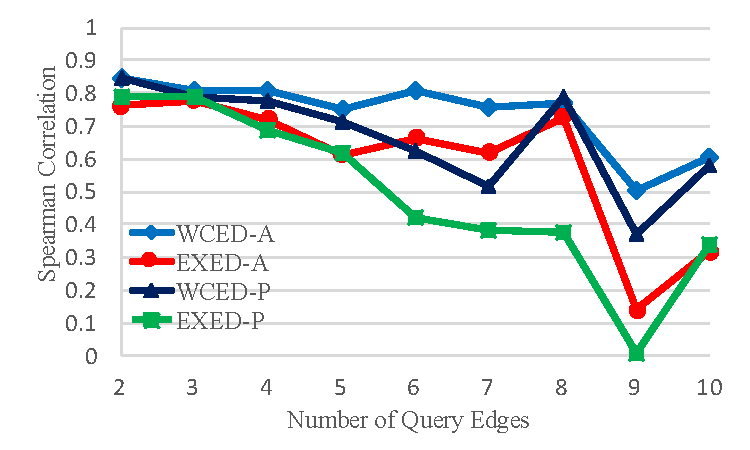
\includegraphics[width=2.5in]{ub_spearman.pdf} 
\caption{Correlation between estimated and actual costs varying the number of query edges}
\label{fig:sel}
\end{figure}

\subsubsection{Upper-bound cost model evaluation}
In this set of experiments, we evaluate the upper bound of cost models of our algorithms presented in Section~\ref{sec:ub}. Let's denote with ``WCED-A" and ``EXED-A'' the upper bounds of the cost model of WCED and EXED assuming independence of adjacent labels respectively, and denote with ``WCED-P" and ``EXED-P'' the upper bounds of the cost model of WCED and EXED assuming independence of path labels respectively. Figure~\ref{fig:sel} shows that both ``WCED-A'' and ``EXED-A'' have a better Spearman correlation with the actual cost than both ``WCED-P'' and ``EXED-P''. Both ``WCED-A'' and ``EXED-A'' have over $0.6$ correlation for queries up to $8$ edges, while ``WCED-P''  only has $0.5$ correlation when queries have $7$ edges and the correlation of ``EXED-P''  drops below $0.4$ when queries have more than $6$ edges. Based on these results, both WCED and EXED using our ``WCED-A'' provide good cost models for comparing the cost of different queries.

Sometimes we have a query and want to find the algorithm that has the least cost before running the algorithms. To evaluate the effectiveness of our cost models, we computed the gaps between the actual costs of WCED and EXED, i.e. actW-actE and their estimated costs, i.e. estW-estE. A high correlation between the two gaps indicates that the cost model can show which algorithm has the least cost even though the actual value of the estimate may not be accurate. Figure ~\ref{fig:costcomp} shows us that for queries with up to $6$ edges, the correlation coefficient is good (over $0.7$). 


\begin{figure}[htbp] 
\setlength{\abovecaptionskip}{-0.5\baselineskip}
\setlength{\belowcaptionskip}{-0.5\baselineskip}
\centering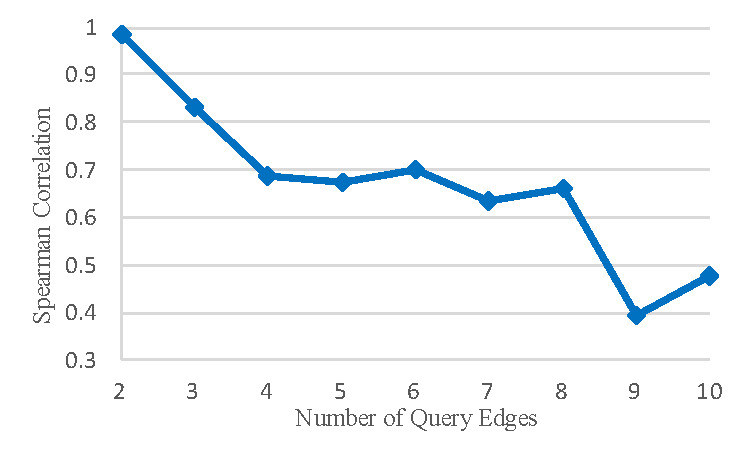
\includegraphics[width=2.5in]{algcostcomp.pdf} 
\caption{Correlation between actual and estimated cost differences varying the number of query edges}
\label{fig:costcomp}
\end{figure}


\subsection{Effectiveness of Our Filtering Strategies}
\label{sec:filtering}
To evaluate the pruning power of our filtering schemes, the number of nodes in the data graph was set to $10$K and the edit distance threshold was set to $1$. Let ``neighbour" denote the neighbourhood-based filtering strategy, ``path" denote the path-based pruning strategy and ``both" denote the case where both schemes were used.

\begin{figure}[htb]
\setlength{\belowcaptionskip}{-1\baselineskip}
\centering
\subfigure{
\centering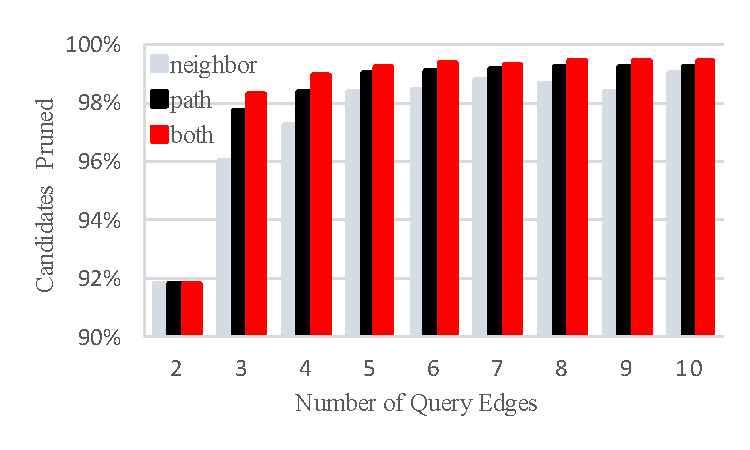
\includegraphics[width=2.7in]{wcprune.pdf}
}
\vspace{-2\baselineskip}

\subfigure{
\centering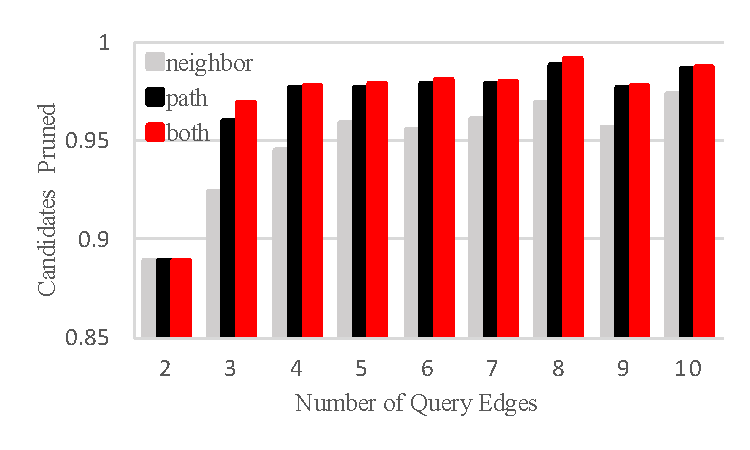
\includegraphics[width=2.7in]{edprune.pdf}
}
\vspace{-2\baselineskip}
\caption{Pruning power of WCED (top) and EXED (bottom) varying the number of query edges}
\label{fig:prune}
\end{figure}

\noindent {\bf Varying the number of query edges:} For this experiment, we varied the number of query edges from $2$ to $10$ and set the edit distance threshold to $1$. Figure ~\ref{fig:prune} shows the fraction of candidates that are pruned in EXED and WCED as we vary the number of query edges.  As shown for WCED and EXED, ``path" can filter out respectively  up to $99.4\%$ and $99.1\%$ of the data nodes on average, while ``neighbour" can filter out respectively up to $99.0\%$ and  $97.3\%$ of the data nodes on average. The pruning power does not increase by more than $1$\% when both strategies are used. However, considering the large number of data nodes and the high cost of verifying each candidate, even a small improvement in the pruning stages is amplified and positively affects the performance of the algorithms (See Figure~\ref{fig:edgenumber}). 
\begin{figure}[htb]
\setlength{\belowcaptionskip}{-1\baselineskip}
\centering
\subfigure{
\centering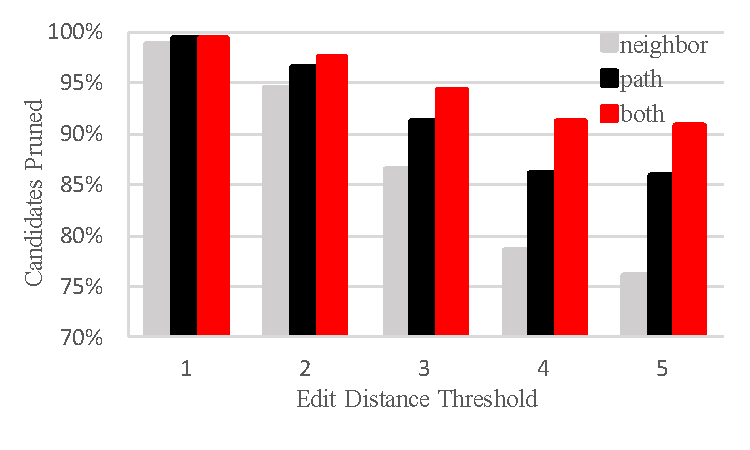
\includegraphics[width=2.8in]{wcthreshold.pdf}
}
\vspace{-2\baselineskip}

\subfigure{
\centering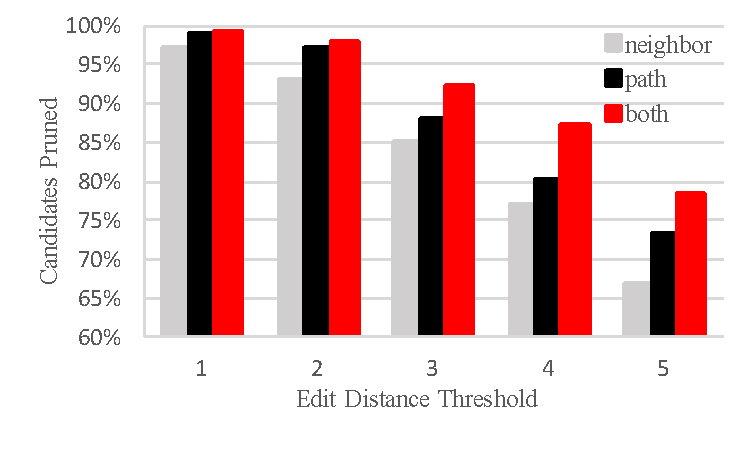
\includegraphics[width=2.8in]{edthreshold.pdf}
}
\vspace{-2\baselineskip}
\caption{Pruning Power of WCED (top) and EXED (bottom) for different edit distance thresholds}
\label{fig:threshold}
\end{figure}


\noindent {\bf Varying the edit distance threshold:} For this experiment, the number of query edges was fixed at $8$ with the edit distance threshold varied from $1$ to $5$. When the edit distance threshold is equal to or exceeds the number of query edges, the labels become irrelevant and the problems becomes subgraph isomorphism on unlabeled graphs, which is not the problem addressed in this paper. Figure ~\ref{fig:threshold} shows that both ``neighbour" and ``path" have good pruning power (over $78\%$) under different distance thresholds, and it becomes more effective to apply both filtering schemes as the edit distance thresholds increases. This is because ``neighbour'' scheme does not encode edge direction in its indexes and higher edit distance threshold introduces more false positives with wrong edge direction, while adding ``path'' on top of ``neighbour'' can effectively prune out those false positives.
\begin{figure}[htb]
\setlength{\belowcaptionskip}{-1\baselineskip}
\centering
\subfigure{
\centering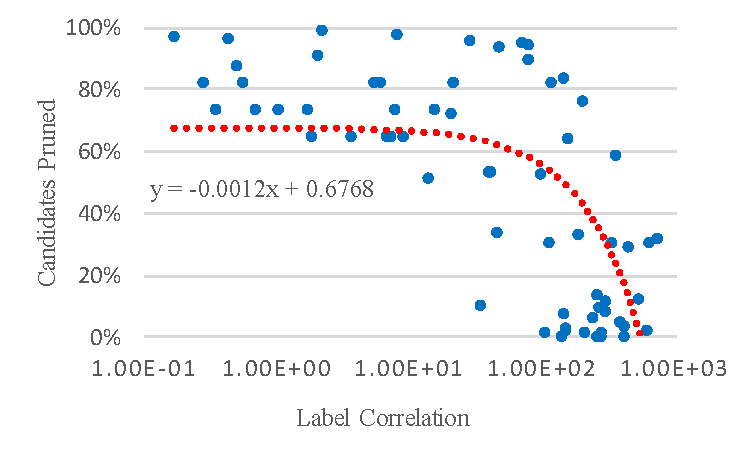
\includegraphics[width=2.7in]{labelcorrelation.pdf}
}
\vspace{-2\baselineskip}

\subfigure{
\centering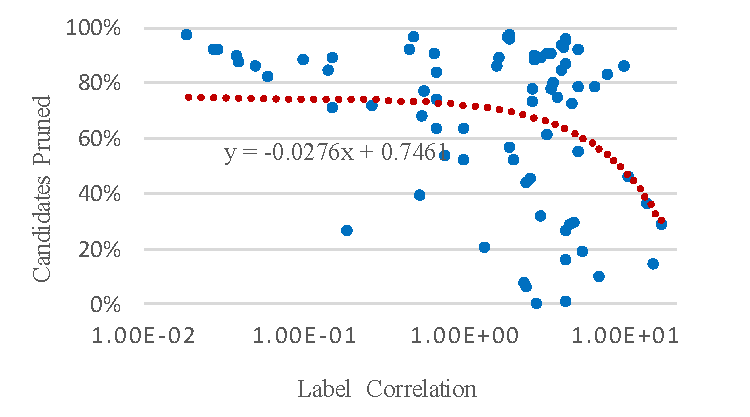
\includegraphics[width=2.7in]{edlabelcor.pdf}
}
\vspace{-2\baselineskip}
\caption{Candidates pruned vs path label correlation of WCED (on the top) and EXED (on the bottom)}
\label{fig:labelcor}
\end{figure}


\noindent {\bf Varying path label correlation:} For this experiment, the neighbourhood filtering scheme is considered as a baseline, on top of which we added our path filtering scheme and monitored the improvement in pruning power. We fixed  the number of query edges at $8$ and set the edit distance threshold to $1$. As shown in Figure~\ref{fig:labelcor} , the improvement in pruning power by adding ``path'' in both EXED and WCED drops with more correlation. This meets our expectation since the more correlated the labels are, the less false positives the neighbourhood-based pruning can produce and the less room for ``path'' filtering improvements.



\begin{comment}
We choose 100 queries with different label correlations. Since the range of label correlation is large, we use log-10 scale for label correlation axis. Figure ~\ref{fig:labelcor} shows that for queries with low label correlation ($\leq 10$), adding path-based pruning algorithm can filter out over  $65\%$ and $70\%$ false positives in WCED and EXED respectively; for queries with  high label correlation ($> 10$), adding path-based pruning algorithm cannot filter out  many false positives in most cases for WCED, while it can filter out  over $60\%$ in most cases for EXED. This meets our expectation. For queries  with low label correlation, the false positives is more than the one for queries with high label correlation. This is because for queries with high label correlation, two labels usually appear together, which results in low false positive rate for pruned candidates with using neighbourhood-based pruning algorithm. For queries with low label correlation,  the appearance of one label is approximately independent of the appearance other labels. In this case, the false positives, which is caused using neighbourhood-based  pruning algorithm, can be relatively high and path-based pruning algorithm is more effective. 
\end{comment}

\begin{comment}
\begin {table}[h]
\begin{center}
\begin{tabular}{ |c|c|c|c| } 
 \hline
  Query edge number& neighbour & bf-path & both \\ 
   \hline
   2&816 & 816&816\\
  \hline
  3 & 434 & 585&429\\ 
   \hline
  4 & 287 & 501&253\\ 
   \hline
  5 & 170 & 402&150\\ 
   \hline
  6 & 160 & 267&141\\ 
   \hline
  7 & 138 & 260&124\\ 
   \hline
  8 & 142 & 243&119\\ 
   \hline
  9 & 173 & 273&143\\ 
   \hline
  10 & 105 & 232&94\\ 
   \hline
\end{tabular}
\end{center}
\caption {WCED candidates number vs different pruning algorithms}
\label{table:wced-pruning}
\end{table}


\begin {table}[h]
\begin{center}
\begin{tabular}{ |c|c|c|c| } 
 \hline
  Query edge number& neighbour & bf-path & both \\ 
    \hline
    2&1115 & 1506 & 1115\\
  \hline
  3 & 768 & 835&676\\ 
   \hline
  4 & 549 & 625&450\\ 
   \hline
  5 & 413 & 589&318\\ 
   \hline
  6 & 446&471&329\\ 
   \hline
  7 & 397&467	&290\\ 
   \hline
  8 & 309	&326	&190\\ 
   \hline
  9 & 433&	565&	360\\ 
   \hline
  10 & 263	&374&180\\ 
   \hline
\end{tabular}
\end{center}
\caption {EXED candidates number vs different pruning algorithms}
\label{table:exed-pruning}
\end{table}

\begin {table}[h]
\begin{center}
\begin{tabular}{ |c|c|c|c| } 
 \hline
  Edit distance & neighbour & bf-path & both \\ 
      \hline
    1&142 & 243 & 119\\
    \hline
    2&170 & 315 & 147\\
  \hline
  3 & 208 & 403&183\\ 
   \hline
  4 & 236 & 449&213\\ 
   \hline
  5 & 306 & 521&281\\ 
   \hline
\end{tabular}
\end{center}
\caption {WCED candidates number vs different distance threshold}
\label{table:wc-threshold-pruning}
\end{table}

\begin {table}[h]
\begin{center}
\begin{tabular}{ |c|c|c|c| } 
 \hline
  Edit distance & neighbour & bf-path & both \\ 
      \hline
    1&309 & 326 & 190\\
    \hline
    2&716 & 636 & 409\\
  \hline
  3 & 1512 & 1573&971\\ 
   \hline
  4 & 2317 & 2400&1577\\ 
   \hline
  5 & 3319 & 2965&2419\\ 
   \hline
\end{tabular}
\end{center}
\caption {EXED candidates number vs different distance threshold}
\label{table:ed-threshold-pruning}
\end{table}
\end{comment}

\subsection{Combining Filtering Schemes}
In these set of experiments, we evaluate the impact of adding path filtering on top of the neighbourhood filtering. In order to show the impact of using both filtering schemes, we consider EXED with the neighbourhood filtering scheme as our baseline and compare it against EXED with both filtering schemes, WCED with the neighbourhood filtering scheme and WCED with both filtering schemes. We denote EXED and WCED with the neighbourhood filtering scheme as ``neighbour-EXED" and ``neighbour-WCED" respectively, WCED and EXED with both filtering schemes as ``both-WCED" and ``both-EXED'' respectively. 

\noindent {\bf Varying the edit distance threshold: }
We varied the edit distance threshold $t$ from $1$ to $5$ and fixed the number of query edges at $8$. Figure~\ref{fig:10ktime} shows that ``neighbour-WCED'' speed ups EXED by a factor of $1.5$ when $t = 5$, reducing the search time more than half in this particular experiment. Comparing ``neighbour-WCED" and ``both-WCED'', we find that even though there is no clear speedup for adding path filtering on top of the neighbourhood filtering scheme at small thresholds ($t \leq 2$), the performance gap becomes wider at larger thresholds with around $200$ seconds saved when $t=5$. This meets our expectation because the benefits of using both schemes over ``neighbour'' in pruning power becomes clear when edit distance threshold increases (See Figure~\ref{fig:threshold}).

\begin{figure}[htbp] 
\setlength{\belowcaptionskip}{-1\baselineskip}
\centering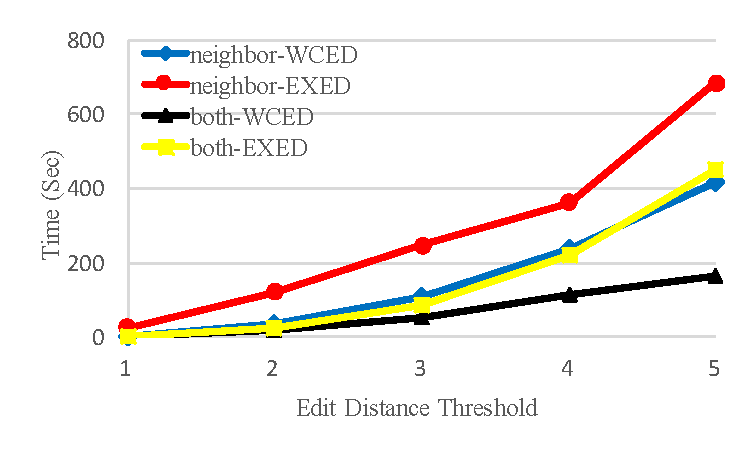
\includegraphics[width=2.5in]{10ktime.pdf} 
\vspace{-1.5\baselineskip}
\caption{Time vs edit distance threshold}
\label{fig:10ktime}
\end{figure}

\noindent {\bf Varying average degree of data graph:} 
In another experiment, we varied the average degree of a node from $5$ to $25$. Figure~\ref{fig:density} shows that ``both-WCED'' has the greater advantage in a data graph with larger average degrees, outperforming ``neighbour-WCED'' and ``neighbour-EXED''. This is because the cost of verifying each candidate depends on the average degree of the data graph, and a larger average degree results in a higher cost of verifying each candidate and thus the wider gap between ``both-WCED'' and the others. 

\begin{figure}[htbp] 
\setlength{\abovecaptionskip}{-0.5\baselineskip}
\setlength{\belowcaptionskip}{-0.5\baselineskip}
\centering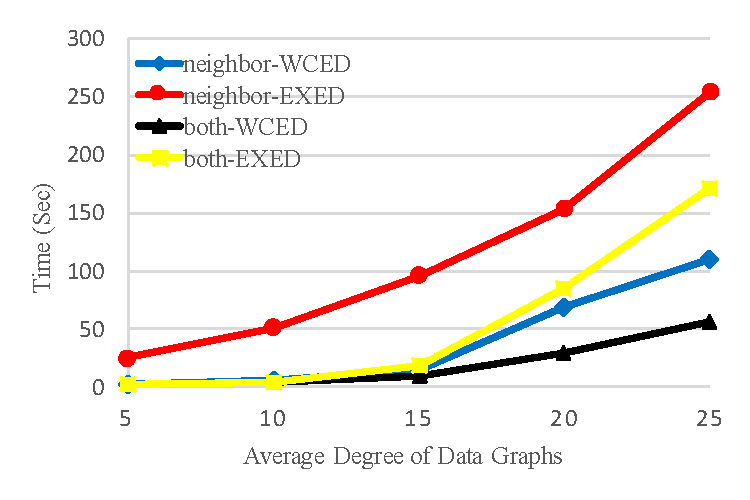
\includegraphics[width=2.5in]{density.pdf} 
\caption{Time vs average degree of data graphs}
\label{fig:density}
\end{figure}

\noindent {\bf Varying the number of query edges:} In another experiment, we varied the number of query edges from $2$ to $10$ with the edit distance threshold fixed at $1$. Figure~\ref{fig:edgenumber} shows that the gap between ``neighbour-WCED'' and ``both-WCED'' (and similarly between ``neighbor-EXED'' and ``both-EXED'') widens as we increase the number of edges. This meets our expectation, because the cost of verifying each candidate grows exponentially with the number of edges. 
\begin{figure}[htbp] 
\setlength{\abovecaptionskip}{-0.5\baselineskip}
\setlength{\belowcaptionskip}{-0.5\baselineskip}
\centering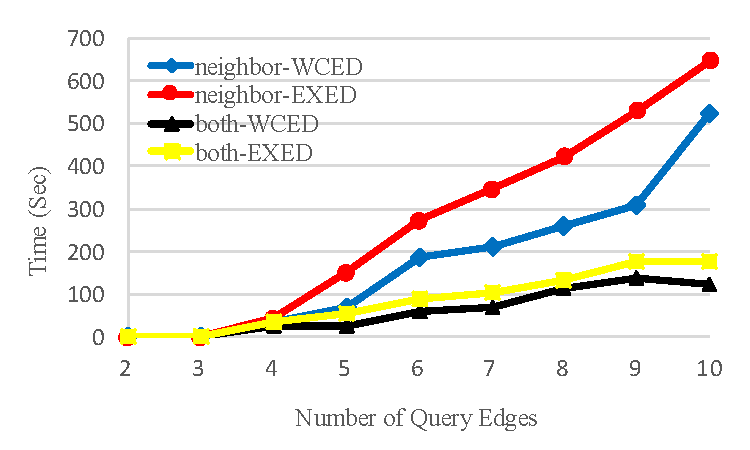
\includegraphics[width=2.5in]{edgenumber.pdf} 
\caption{Time vs number of query edges}
\label{fig:edgenumber}
\end{figure}

Our experiments in this section reveals that adding path filtering improves the performance of both algorithms EXED and WCED under one or more of these conditions: (1) the data graph has high average degree; (2) the edit distance threshold $t \geq 2$; (3) the query has over $5$ edges. 

\subsection{Algorithms Comparison}
\label{sec:comp}
To evaluate the performance of our algorithms against the competitors, we selected two recent algorithms from the literature: (1) SAPPER~\cite{zhang2010sapper} which is an algorithm for indexing and approximate matching in large graphs, and (2) Exemplar~\cite{mottin2014exemplar} which is similar to our work but is limited to edit distance threshold zero.  

\noindent {\bf Comparing against SAPPER:} 
In this experiment, we compare the scalability of our algorithms against SAPPER. We varied the number of nodes in the data graph from $1$K to $100$K and set the edit distance threshold to $1$. This is consistent with the settings by the authors of SAPPER except that their largest data graph had only $10$K nodes. 
Since SAPPER only supports edge deletion (missing edges), we modified SAPPER to support edge label substitutions. The running time for SAPPER and our algorithms is reported in Figure~\ref{fig:comp}. The Figure shows that the running time of SAPPER grows much faster than our algorithms. We also observe that our algorithms are not very sensitive to the changes in the size of the data graph. WCED with both filtering schemes shows the best performance. 
\begin{figure}[htbp] 
\setlength{\abovecaptionskip}{-0.5\baselineskip}
\setlength{\belowcaptionskip}{-0.5\baselineskip}
\centering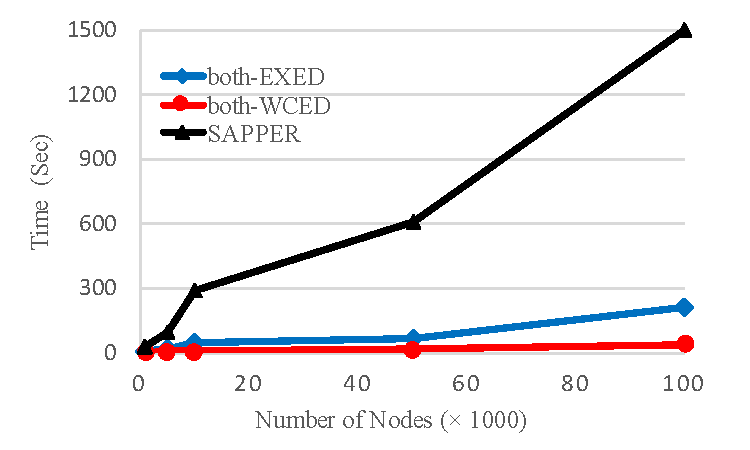
\includegraphics[width=2.5in]{comp.pdf} 
\caption{Time vs different algorithms}
\label{fig:comp}
\end{figure}

\noindent {\bf Comparing against Exemplar queries:} 
To evaluate the effectiveness of our queries and to compare them to the exemplar queries of Motin et al.\cite{mottin2014exemplar}, we chose $10$ queries from the AOL query log and manually mapped them to subgraphs in freebase. The chosen queries are listed in the Appendix of \cite{eteq2016}. The number of query edges ranged between $4$ and $8$. To control the size of the answer set (and to avoid a blow-up), we varied the edit distance threshold from $0$ to $2$. When the edit distance threshold is $0$, our queries are identical to exemplar queries. As expected and shown in Figure~\ref{fig:exqcomp}, the larger the edit distance thresholds are, the more answers are returned.
\begin{figure}[htbp] 
\setlength{\abovecaptionskip}{-0.5\baselineskip}
\setlength{\belowcaptionskip}{-0.5\baselineskip}
\centering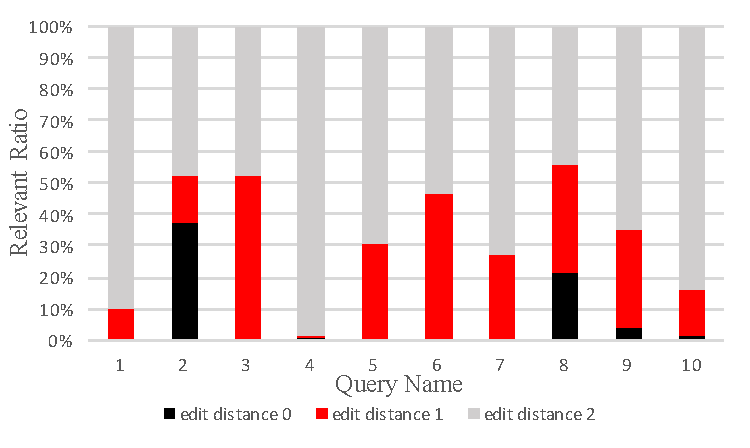
\includegraphics[width=2.5in]{exqcomp.pdf} 
\caption{Answer set composition}
\label{fig:exqcomp}
\end{figure}

To evaluate the quality of ETEQ answers, we conducted the following user study. We asked 10 users (uniformly distributed with respect to education level, age and country) to evaluate our system. For each query in the test set, we provided an explanation of the topic, the query intention, and our answer set with different edit distances. We asked each user to rate each result as irrelevant or relevant with respect to the topic and the expressed query intent. Due to the large size of the answer sets, for each answer set and each edit distance, we randomly chose up to $10$ answers for evaluation. Figure~\ref{fig:relevance} shows that the ratio of relevant answers to all returned answers decreases as the edit distance threshold increases. This meets our expectation, since the more edit operations are allowed, the less number of relevant answers are expected to be returned. We also observe in Figure~\ref{fig:exqcomp1} that the relevant set has many answers with edit distances $1$ and $2$. These answers cannot be returned by exemplar queries. 


\begin{figure}[htbp] 
\setlength{\abovecaptionskip}{-0.5\baselineskip}
\setlength{\belowcaptionskip}{-0.5\baselineskip}
\centering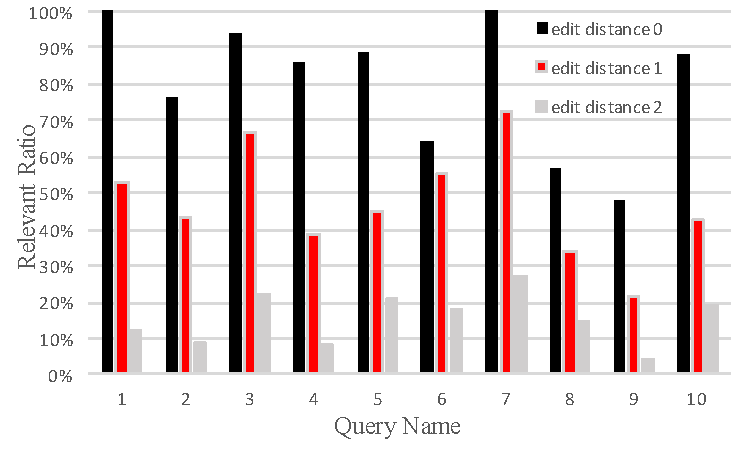
\includegraphics[width=2.5in]{relevance.pdf} 
\caption{Relevance for each edit distance}
\label{fig:relevance}
\end{figure}

\begin{figure}[htbp] 
\setlength{\abovecaptionskip}{-0.5\baselineskip}
\setlength{\belowcaptionskip}{-0.5\baselineskip}
\centering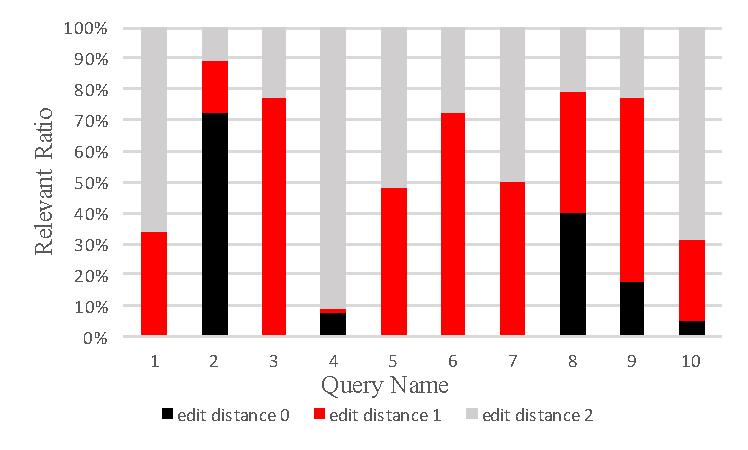
\includegraphics[width=2.5in]{exqcomp1.pdf} 
\caption{Relevant answer set compostion}
\label{fig:exqcomp1}
\end{figure}

We are not comparing the efficiency of our algorithms against Exemplar because (1) Exemplar does not support edit distance thresholds larger than zero, and (2) our EXED algorithm becomes identical to Exemplar when the edit distance threshold is zero and we have extensively evaluated EXED with different edit distance thresholds.

\section{Related Work}
\begin{comment}
The first category of related research lies in subgraph isomorphism algorithms. Ullmann firstly proposed a s a recursive backtracking procedure for solving the subgraph isomorphism problem. VF2, QuickSI , GraphQL, GADDI, and SPath have been proposed to improve the performance of the Ullmann algorithm. These algorithms exploit different join orders, pruning rules, and auxiliary information to prune out false positive candidates as early as possible, thereby increasing performance.
 \end{comment}
The problem of subgraph isomorphism is NP-complete and this is a special case of graph edit distance with the edit distance threshold set at zero. Most existing methods adopt a filter-and-verification framework. Wang et. al.\cite{wang2012efficiently} propose  an efficient index for sparse data graphs. They decompose graphs to small grams (organized by $\kappa$-Adjacent Tree patterns) and uses these $\kappa$-AT patterns to estimate a lower bound of their edit distance for candidate filtering. Zeng et. al. \cite{zeng2009comparing} propose another method to compute the edit distance by transforming a graph to a multi-set of star structures. Zheng et. al.\cite{zeng2009comparing} proposed a path-based index for candidates filtering. However, all these algorithms are targeting  data graphs that are small ($<$ $10$K nodes), sparse and are not suitable for discovering information from RDF data graphs such as freebase.
 
Approximate graph matching or similarity based search in large graphs has been studied in the past under various settings. TALE\cite{tian2008tale} introduces a neighbourhood based index (NH-Index) where it matches important vertices of a query graph first before extending the match progressively. SAPPER\cite{zhang2010sapper} takes advantage of pre-generated random spanning trees and a carefully designed graph enumeration order to find approximate subgraph matches.  Mongiovi et. al.\cite{mongiovi2010sigma} introduced a set-cover based inexact subgraph matching technique, called SIGMA. Most of these algorithms are designed to find part (e.g. Top-k) of approximate matches and may use their own similarity measures. 


Our approach is related to works in  which the query node's neighbourhood information is used to prune graph candidate nodes that  are not related to those in the query\cite{khan2011neighborhood}. Our experiments confirm that combining both indexes performs better than either index alone. Our work is also related to exemplar queries in the way that we both find relevant answers with similarity measure based on edge label. Exemplar queries can only find relevant answers that are edge-isomorphic to the query, while our algorithms in this paper can find relevant subgraphs that are edge-preserving isomophic to the query after some edit operations. 

\section{Conclusion}
In this paper, we study the problem of error-tolerant exemplar queries on RDF graph. Unlike exemplar queries that supports only exact matching of the labels, our developed algorithms allow errors in  query and data graph. Two filtering techniques (neighbourhood and path filtering) and two algorithms (EXED and WCED) are developed to handle edit operations as well as to facilitate the searching process. Through a comprehensive experimental evaluation on real and synthetic datasets, we show that our algorithms are both efficient and effective, outperforming existing algorithms.  As a future work, we plan to efficiently support Top-k queries. 
%\bibliographystyle{plain}
%\bibliography{sigmod.bib}
%
% The following two commands are all you need in the
% initial runs of your .tex file to
% produce the bibliography for the citations in your paper.
\def\thebibliography#1{
    \section*{References}
    %\normalsize
    %\small
    \footnotesize
    %\scriptsize                  % smaller; put \normalsize after bib --dt
    \list
    {[\arabic{enumi}]}
    {\settowidth\labelwidth{[#1]}
        \leftmargin\labelwidth
        \parsep 0pt                % tighter --dt
        \itemsep 0pt              % tighter --dt
        \advance\leftmargin\labelsep
        \usecounter{enumi}
    }
    \def\newblock{\hskip .11em plus .33em minus .07em}
    \sloppy\clubpenalty10000\widowpenalty10000
    \sfcode`\.=1000\relax
} 

\bibliographystyle{abbrv}
\bibliography{sigmod}  % sigproc.bib is the name of the Bibliography in this case
% You must have a proper ".bib" file
%  and remember to run:
% latex bibtex latex latex
% to resolve all references
%
% ACM needs 'a single self-contained file'!
%
%APPENDICES are optional
%\balancecolumns
\appendix
%Appendix A
\section{Proof of Lemma}
\subsection{Proof of Lemma 1}
\begin{proof}
This lemma can be proved using the probability subtraction rule:
%% CHANGE to P_D
\begin{align}
&P_D(l_1, l_2, ..., l_k) = \nonumber \\
&P_D(l_2, ...,l_k) - P_D(\neg l_1, l_2, ..., l_k)= \nonumber \\
&P_D(l_2, ...,l_k) - (P_D(\neg l_1, l_3, \ldots, l_k) - P_D(\neg l_1, \neg l_2, ..., l_k))= \nonumber \\
&P_D(l_2, l_3, ...,l_k) - P_D(\neg l_1, l_3, \ldots, l_k) + P_D(\neg l_1, \neg l_2, l_4, \ldots, l_k) \nonumber \\
&- P_D(\neg l_1, \neg l_2, \neg l_3, ..., l_k)= \nonumber\\
&...\nonumber\\
&\sum_{i=2}^k (-1)^{i-1}P_D(\neg l_j,\ldots,\neg l_{i-1}, l_{i+1}, \ldots, l_k)\nonumber\\
&+ (-1)^k P_D(\neg l_1, \neg l_2, ..., \neg l_k) + P_D(l_2, l_3, ...,l_k).
\label{eq:P_Dderive}
\end{align}
 
If we expand $P_D(l_2,\ldots,l_k)$ further using the equation above, we will have a set of terms that look similar to the first and the second terms in Eq~\ref{eq:P_Dderive} and the base case $P_D(l_k)$. For the base case, we have $P_D(l_k)=(1-(1-Sel(l_k))^D$. We also know that $P_D(\neg l_j, \ldots, \neg l_k)=(1-\sum_{i=j}^k Sel(l_i))^D$ assuming independence. Putting these pieces together will give the statement of the lemma.

%This completes the proof.
\end{proof}

\subsection{Proof of Lemma 2}
\begin{proof}

Using Equations~\ref{eq:cost-verifying-n}, the cost of verifying each wildcard queries for WCED with edit distance $1$ can be written as
\begin{align*}
Cost_{wc} =\sum_{k = 1}^{|E_q|}\sum_{i=1}^{|E_q|}\prod_{j = 1}^i\hat{D}*Sel(l_{k,j})
\end{align*}

Let $l_1,\ldots,l_k$ denotes the labels in increasing order of selectivities. Since the edges in a query are verified in increasing order of selectivities, for those wildcard queries where $l_j (1\leq j \leq i)$ is not set to wildcard, the edge with label $l_i$ is verified at $i^{th}$ step of the simulation,  the cost of verifying the edge is $\hat{D}^i\prod_{j=1}^iSel(l_j)$, there are $|E_q| - i$ these type of wildcard queries; for those that $l_j (1\leq j \leq i)$ is set to wildcard, the edge with label $l_{i+1}$ is verified at $i^{th}$ step of the simulation, the cost of verifying this edge is $\hat{D}^i\prod_{j=1}^{i+1}Sel(l_j)$, where $l_j \not= l_m$. 

Let $T_i$ be
\begin{equation}
\label{eq:tl}
T_i = \sum_{k=1}^{i} \prod_{m=1}^{i} Sel(l_{k,m}) \text{ where } l_{k,m} \not= l_k.
\end{equation}

The sum of verifying costs for those wildcard queries that $l_m (1\leq m \leq i - 1)$ is set to wildcard at $i^{th}$ step of the simulation is $\hat{D}^i(T_{i+1} - \hat{D}^i\prod_{j=1}^{i-1}Sel(l_j))$.
Then, the sum of verifying costs for WCED can be written as 
\begin{align*}
Cost_{wc}&=\sum_{i=1}^{|E_q| - 1}\hat{D}^i((|E_q| - i - 1)\prod_{j=1}^i Sel(l_j) + T_{i+1})\\
&+\hat{D}^{|E_q|}T_{|E_q|}.
\end{align*}

Using Equations~\ref{eq:st-cases} and~\ref{eq:ed-verify}, the verifying cost of EXED with edit distance threshold $1$ can be written as 
\begin{align*}
Cost_{ex}&=\hat{D} + \sum_{i=2}^{|E_q|}(\hat{D}^{i}\sum_{k=1}^{i-1} (1 - Sel(l_k))\prod_{j=1}^{i}Sel(l_{k,j})\\
&+ \hat{D}^{i}\prod_{j=1}^{i-1}Sel(l_j)), \text{where } l_{k,j} \not= l_k
\end{align*}
Replacing the terms in above equation with Equation~\ref{eq:tl}, $Cost_{ex}$ can be written as
\[
Cost_{ex}=\hat{D} + \sum_{i=2}^{|E_q|}\hat{D}^{i}(T_{i} - (i-1)\prod_{j=1}^{i}Sel(l_j))
\] 
Then, the difference between two costs $\Delta_{cost}$ can be written as
\begin{align*}
&\Delta_{cost} = \hat{D}(1 - (|E_q| - 1)Sel(l_1) - Sel(l_2)) \\
&+ \sum_{i=2}^{|E_q| - 1}\hat{D}^i(T_i - T_{i+1} -  (|E_q| - 2)\prod_{j=1}^i Sel(l_j))\\
&- (|E_q| - 1)\hat{D}^{|E_q|}\prod_{i=1}^{|E_q|}Sel(l_i).
\end{align*}
Since query edges are visited in increasing order of label selectivities, we have an inequality as follows
\[
Sel(l_1) \leq Sel(l_i) \leq 1.
\]
With the inequality above, we have 
\[
iSel(l_1)^{i-1}\leq T_i \leq i
\]
Using the both inequalitis above, the upper bound of $\Delta_{cost}$ can be written as
\begin{align*}
&\Delta_{cost} \leq \hat{D}(1 - {|E_q|}Sel(l_1)) - (|E_q| - 1)\hat{D}^{|E_q|}Sel(l_1)^{|E_q|}\\
&+ \sum_{i=2}^{|E_q| - 1}\hat{D}^i(i -(|E_q| + i - 1) Sel(l_1)^i).
\end{align*}
Let $F_n(x)$ denote the upper bound of $\Delta_{cost}$ using $x$ to denote $Sel(l_1)$ and $n$ to denote the number of query edges. To show the correctness of the Lemma~\ref{lemma:comp}, we prove that $F_{|E_q|}(x) \leq 0$ with different number of edges when the conditions in the Lemma holds using mathematical induction.
\basis
$n = 2$: $F_2(x)$ can be written as 
\[
F_2(x) = \hat{D}(1 - 2x) - \hat{D}^2x^2
\]
When $x = \frac{1}{\sqrt{\hat{D}}}$, we have $F_2(x)$.
\[
\hat{D}(1 - 2x) - \hat{D}^2(\frac{1}{\sqrt{\hat{D}}})^2 = \hat{D}(-2x)<0.
\]
We also know that the derivative of $F_2(x)$ is
\[
\frac{\partial F_2}{\partial x} = -2\hat{D} - 2\hat{D}^2x < 0.
\]
Combining two facts above, we know that $F_2(x) < 0$ when $Sel(l_1) > \frac{1}{\sqrt{\hat{D}}}$.
\ih
the Lemma holds when the query has $k$ edges.
\begin{align*}
F_k(x) &= \hat{D}(1 - kx) - (k - 1)\hat{D}^kx^k\\
&+ \sum_{i=2}^{k - 1}\hat{D}^i(i -(k + i - 1) x^i) < 0\\
& \text{subject to }  x > \frac{1}{\sqrt[k]{\hat{D}}}.
\end{align*}
Note that the derivative of  $F_k(x)$ is
\[
\frac{\partial F_{k}}{\partial x}= -k - k(k-1)\hat{D}^kx^{k-1}-\sum_{i=2}^ki(k+i-1)x^{i-1} < 0.
\]
\is Using $F_k(x)$ to substitute some terms in $F_{k+1}(x)$,  $F_{k+1}(x)$ can be written as
\begin{align*}
&F_{k+1}(x) = \hat{D}(1 - (k+1)x) - k\hat{D}^{k+1}x^{k+1}\\
&+ \sum_{i=2}^{k}\hat{D}^i(i -(k + i ) x^i) =\\
 &F_k(x) - \hat{D}x -  \sum_{i=2}^{k-1}x^i + D^k(k - (k+1)x^k) + k\hat{D}^{k+1}x^{k+1}.
\end{align*}
When  $x = \frac{1}{\sqrt[k+1]{\hat{D}}}$, after replacing the $x$ with the value in the last term and combining the last two terms, $F_{k+1}(x)$ can be written as
\begin{align*}
&F_{k+1}(\frac{1}{\sqrt[k+1]{\hat{D}}}) = F_k(x) - \hat{D}x -  \sum_{i=2}^{k-1}x^i + D^k(k - (k+1)x^k) \\
&+ k\hat{D}^{k+1}(\frac{1}{\sqrt[k+1]{\hat{D}}})^{k+1} = F_k(x) - \hat{D}x -  \sum_{i=2}^{k-1}x^i -(k+1)D^kx^k
\end{align*}
Since $x = \frac{1}{\sqrt[k+1]{\hat{D}}} > \frac{1}{\sqrt[k]{\hat{D}}}$, $F_k(x) < 0$ and the rest of terms are also negative, we have
\[
F_{k+1}(\frac{1}{\sqrt[k+1]{\hat{D}}}) < 0.
\]
We also know that the derivative of $F_{k+1}(x)$ is negative. 
\[
\frac{\partial F_{k+1}}{\partial x} = \frac{\partial F_{k}}{\partial x} - \hat{D} - \sum_{i=2}^{k-1}ix^{i-1} - k(k+1)\hat{D}^kx^{k-1} < 0.
\]
Combining two facts above, we know that $F_{k+1}(x) < 0$ when $Sel(l_1) > \frac{1}{\sqrt[k+1]{\hat{D}}}$.
\end{proof}
\section{Query Set}
The query set used to compare with exemplar queries in Section ~\ref{sec:comp} with format ``<subject> <predicate> <object>'' as follows:
\begin{enumerate}
\item D influenced Swift;\\
Scala influenced Swift;\\
Ruby influenced Swift;\\
Rust influenced Swift;\\
Swift languages Function programming;\\
Swift languages Procedural programming;\\
Swift languages Generic programming;\\
Swift subject\_of Treehouse.
\item Lloyd Wright structures\_designed Oasis Hotel;\\
Lloyd Wright place\_of\_death Santa Monica;\\
Lloyd Wright architectural\_style Modern architecture;\\
Lloyd Wright influenced\_by Frederick Law Olmsted;\\
Lloyd Wright influenced\_by Frank Lloyd Wright.
\item National Audubon Society notable\_types Nonprofit organization;\\
National Audubon Society program\_partnership\_s Appalachian Mountains Joint Venture;\\
National Audubon Society program\_partnership\_s Virginia Bird Conservation Initiative;\\
National Audubon Society named\_after John James Audubon.
\item Pythagoras namesakes Pythagoras;\\
Pythagoras influenced Nikohl Vandel;\\
Pythagoras children Damo;\\
Pythagoras influenced Plato;\\
Pythagoras influenced Jābir ibn Hayyān.
\item Frederick County contains Ole Orchard Estates;\\
Frederick County events Second Battle of Winchester;\\
Frederick County partially\_contains North Mountain;\\
Frederick County contains Echo Village;\\
Frederick County people\_born\_here James Brenton (1740–1782);\\
Frederick County contains Green Acres;\\
Frederick County contains US Census 2000 Tract 51069050100.
\item Research subject\_of Carnegie Moscow Center;\\
Research works Hot talk, cold science;\\
Research works Person or Persons Unknown;\\
Research organizations\_of\_this\_type Stanford University School of Medicine;\\
Research schools\_of\_this\_kind Indian Institute of Forest Management;\\
Research organizations\_of\_this\_type Stanford Radiology.
\item Valve Corporation games\_developed Half-Life 2;\\
Valve Corporation games\_published Wolfenstein 3D;\\
Valve Corporation games\_published The Maw;\\
Valve Corporation games\_developed CS Online;\\
Valve Corporation games\_published Half-Life 2;\\
Valve Corporation is\_reviewed Place founded;\\
Valve Corporation games\_published CS Online.
\item Scheme influenced Haskell;\\
Scheme influenced Clojure;\\
Scheme influenced LFE;\\
Scheme influenced Dylan;\\
Scheme influenced\_by Lisp;\\
Scheme parent\_language Lisp.
\item Cruze Control genre Southern hip hop;\\
Cruze Control notable\_types Musical Album;\\
Southern hip hop artists Triple C's;\\
Cruze Control featured\_artists Baby;\\
Cruze Control featured\_artists Pitbull;\\
Southern hip hop albums Cruze Control.
\item Luke Carroll place\_of\_birth Sydney;\\
Marcus Einfeld place\_of\_birth Sydney;\\
Martin Lynes place\_of\_birth Sydney;\\
George Tarr place\_of\_birth Sydney;\\
Adventures by Disney \- Australia Vacation travel\_destinations Sydney;\\
Dayne Hudson place\_of\_birth Sydney.
\end{enumerate}

%\balancecolumns % GM June 2007
% That's all folks!
\end{document}